\documentclass[11pt]{article}
\usepackage[margin=1in]{geometry}
\usepackage{graphicx,booktabs,amsmath,longtable}
\usepackage[round,authoryear]{natbib}
\usepackage[hidelinks]{hyperref}
\title{Catalog observations and limits on reproducing earthquake-triggered activity at Sierra Negra}
\author{Reproducibility project}
\date{9 October 2026}
\begin{document}
\maketitle
\begin{abstract}
Earthquake timing and waveform recurrence can constrain the processes connecting fault slip to eruption. We assess the reproducibility of Song et al. (2026) and calculate seismicity statistics from the independently archived original catalog. The full archived catalog passes its published checksum and contains 219 earthquakes on 26 June 2018. Their distribution among four published activity windows is 29, 74, 72, and 44 events. We implement and test spectral classification, signed cross-correlation, connected-component clustering, magnitude-to-moment conversion, and recurrence statistics. We acquire nine three-component seismic station records, eight complete and one gapped, and execute a public picker on the seven 8G stations producing 6,908 P and 6,379 S candidates, review the supplementary methods, and independently process four historical PAYG day plots. We independently process both GNSS records with RTKLIB float PPP; the one-hour mean vertical change at GV09 is 1.867 m, consistent with the published lower bound of 1.83 m. Missing station records and source controls prevent exact association and relocation reproduction; a published Sierra Negra 1-D model supports 536 explicitly approximate candidate locations. A seven-station template search with 447 templates adds 1,007 candidates, yielding 1,543 candidates with inherited classifications of 453 LP and 1,088 VT events and two unclassified events. These independently computed candidates are not the source relocated catalog. Exact multiplet membership and published regression agreement remain unverified. Partial observation-based figures and an original conceptual schematic document the available calculations. The results establish a reusable numerical basis and a transparent assessment of missing inputs; they do not independently verify a fluid-triggering mechanism.
\end{abstract}

\section{Introduction}
Volcanic eruption initiation involves mechanical interaction between a magma reservoir and the surrounding faulted edifice. Seismic timing alone leaves an ambiguity: fault slip may open a magma pathway directly, or it may initiate a sequence of processes that eventually permits intrusion. The Sierra Negra observations motivate testing this distinction because a well-recorded fault earthquake preceded the 2018 eruption \citep{bell2021,song2026}.

An enhanced earthquake catalog can reveal signals absent from an original monitoring catalog, but agreement depends on waveform coverage, detection thresholds, and manual decisions. We distinguish three reproducibility questions: whether an archived original catalog can be recovered; whether numerical components behave as defined; and whether the enhanced observations and mechanism can be independently verified. The first two questions are addressed directly; approximate association and independent GNSS calculations address parts of the third. The project assessment explicitly retains the third as unresolved.

\section{Data availability and provenance}
The original earthquake catalog is deposited with geodetic and interferometric products by \citet{bellarchive}. We downloaded the complete event list and verified its published MD5. The date-specific subset confirms all 219 previously recovered browser rows. It retains identifiers, origin times, coordinates, catalog depths, magnitudes, location-error fields, travel-time RMS, azimuthal gap, and phase-pick counts. Full-source SHA-256 and archive provenance accompany the derived catalog. Zenodo metadata specify CC-BY-4.0 licensing. The archived long-term GNSS baseline also passes its published checksum but does not replace high-rate positions.

Public metadata identify IGUANA as network 8G during 2018--2019 \citep{iguana}. Network access permits downloading 21 complete 100-Hz channels from seven 8G stations: SN04, SN05, SN07, SN11, SN12, SN13 and SN14. Two additional EC station records are acquired with responses: SN06 is complete, while SN02 has 79,636.67 seconds of common three-component coverage (92.172\%). A consolidated map displays fourteen seismic metadata stations, distinguishing the nine acquired stations from metadata-only entries. Missing records remain a coverage limitation. The public Volpick repository provides trained models \citep{volpick,zhong2024}, and public checkpoint v1 is downloaded on the data drive. Its equivalence to the authors' checkpoint is unverified. The separate VCH1 original catalog passes its published checksum and contains 191 entries on the date; it is not merged with the located catalog because event equivalence is unverified. The archived scalar GNSS baseline is acquired; independent high-rate positions are subsequently calculated from authenticated RINEX observations. The full archived VCH1 catalog also matches its published checksum and contributes 191 entries on the date. These time/magnitude entries remain separate from the 219 located events because shared event identities and locations are unavailable for reliable merging. Authenticated EarthScope retrieval supplies GPS RINEX 2.11 observations and station-specific navigation records for GV03 and GV09. GV09 has all 2,880 daily 30-second epochs; GV03 has 1,431 and a 03:21:42--12:46:12 UTC gap spanning the fault earthquake. GPS observation times are converted to UTC using the header 18-second offset.

The accessible main article does not expose a separate Code Availability section or an enhanced catalog download. Targeted searches did not identify a study-specific code deposit. This does not establish that such a deposit is absent. The supplementary PDF is downloaded and its methods, equations and nine figures are reviewed. Picking uses 100-Hz inputs filtered at 2--12 Hz, 60-second windows with 50\% overlap and 0.2 phase thresholds. Association requires four P and one S arrival with a 0.5-second residual tolerance. The cited velocity-model manuscript \citep{rezaeifar2024} displays a P model but does not provide numerical layer values identified in the accessible text. We use independently published P and S values from Tepp et al. (2014), Table 1, Model F, as an explicitly approximate alternative \citep{tepp2014}.

\section{Methods}
\subsection{Original-catalog calculations}
We parse source rows without rejecting events by location uncertainty, magnitude, or depth. Validation requires unique identifiers, finite numerical fields, valid coordinate ranges, and chronological ordering. UTC boundaries of 09:15, 17:00, and 19:40 define half-open phase intervals. An event exactly on a boundary belongs to the later phase. This uses the publication's rounded times; the largest catalog event occurs 32.299 seconds after the first boundary and is consequently counted in Phase 2.

For phase $k$, the observed catalog rate is $r_k=N_k/\Delta t_k$, where $N_k$ is the number of catalog entries and $\Delta t_k$ is the interval duration in hours. This rate describes the catalog. It is not corrected for completeness, missing stations, or time-dependent noise. Maps preserve source coordinates; zoomed panels state how many events lie outside their extent. The latitude--depth plot includes every event rather than imposing an undocumented cross-section selection. The source depth datum is not verified, so the plotted values are labeled catalog depth.

\subsection{Waveform and classification components}
Waveform processing requires contiguous finite segments. The implementation rejects gaps instead of silently filling them. Detrending, Butterworth bandpass filtering, and rational anti-alias resampling are available, but filter order and phase convention must be specified. Instrument-response removal is a dependency-bound ObsPy operation with an explicit stabilization passband. None of these operations were applied to Sierra Negra waveforms in this run.

The classification kernel calculates
\begin{equation}
 F=\log_2\left(\frac{\overline{A}_{9\text{--}15}}{\overline{A}_{2\text{--}5}}\right),
\end{equation}
where $\overline{A}$ is mean Fourier amplitude in the indicated frequency band, in hertz. Five-second arrival windows can be extracted from one second before a pick. This expression measures amplitude contrast; it is not an integrated power ratio. Station estimates are averaged only when their supplied signal-to-noise ratios satisfy the criterion of two. Values below $-2$ are LP, and values at or above $-2$ are VT. Missing measurements remain unclassified. These definitions follow the accessible method description \citep{song2026}; taper, SNR definition, and filter details remain unresolved.

\subsection{Correlation and families}
Continuous template correlation uses FFT convolution through compiled SciPy routines. Moving-window sums and sums of squares give the local normalization. Constant templates and non-finite samples are rejected; zero-energy data windows return undefined scores. Detection requires explicit thresholds and separation. We implement both absolute and the EQcorrscan median-absolute-score convention \citep{eqcorrscan}; a chosen sensitivity threshold would not be labeled a published threshold.

An independent C++ kernel demeans each overlapping event-pair window, computes normalized cross-correlation at a user-specified range of integer lags, and retains the sign of the coefficient with largest absolute value. Thus a polarity-reversed signal remains negatively correlated. Common station/component/phase windows contribute to a network average; missing channels contribute no artificial zero. This equal-channel weighting and lag selection are independent conventions awaiting comparison with supplementary details.

Positive network coefficients greater than 0.7 create graph edges. Connected components with at least ten events define candidate families; explicit template links can propagate family and FI membership. Negative coefficients below $-0.7$ create review candidates, not automatically confirmed anti-repeaters. Observed polarity reversals require station-by-station inspection. We construct observational graphs on the seven-station candidates and the template-expanded population, using an independently specified four-common-station quality screen and a 0.2-s maximum lag.

\subsection{Recurrence, moment, and geodesy}
For chronologically ordered family events, recurrence intervals are $T_i=t_{i+1}-t_i$. Periodicity is their mean divided by their standard deviation. The implementation exposes the population versus sample standard-deviation choice because that convention is not resolved. Duplicated origin times require review.

The accessible moment conversion is
\begin{equation}
 M_0=10^{1.5 M_w+9.105}\ \mathrm{N\,m},\qquad
 M_w=\begin{cases}M_L,&M_L>3,\\2M_L/3+1,&M_L\leq3.\end{cases}
\end{equation}
Its application to a new catalog requires confirming the magnitude scale. The regression functions require explicit linear or logarithmic coordinates and an explicit choice of pairing moment with the preceding or following recurrence interval. Leave-one-out jackknife calculations estimate slope variability. These choices cannot be selected by optimizing agreement with a target coefficient.

The geodetic differencing utility averages positions in one-hour windows before and after an earthquake; the independent RTKLIB calculation described below supplies those positions. A full geodetic reproduction requires observations, correction products, software, and control settings. Executed approximate association uses published 1-D P/S velocities \citep{tepp2014,pyocto}; differential relocation still requires input controls and observations \citep{waldhauser2001}.

\section{Results}
The recovered original catalog contains 219 earthquakes, with a magnitude range from $-0.63$ to 4.73 and median 1.78. The largest entry, dias2018mkgw, has an origin time of 09:15:32.299 UTC. Its catalog magnitude is retained as 4.73; it is not substituted for the separately reported moment magnitude of the fault earthquake.

\begin{table}[ht]
\centering
\begin{tabular}{lrrrr}\toprule
Phase & Duration (h) & Events & Rate (h$^{-1}$) & Median magnitude\\\midrule
1 & 9.250 & 29 & 3.135 & 0.900\\
2 & 7.750 & 74 & 9.548 & 0.845\\
3 & 2.667 & 72 & 27.000 & 2.935\\
4 & 4.333 & 44 & 10.154 & 2.520\\\bottomrule
\end{tabular}
\caption{Calculations from the original archived catalog. UTC boundaries are 00:00, 09:15, 17:00, 19:40, and 24:00. Counts include all source events and are not completeness-corrected.}
\label{tab:phases}
\end{table}

Figure~\ref{fig:map} shows the spatial observations recoverable without waveform processing. One location lies far from the caldera vicinity; preserving it makes the distinction between source data and an interpreted local population explicit. No new location inversion or structural reconstruction is implied. Figure~\ref{fig:timeline} and Table~\ref{tab:phases} show the highest observed catalog rate during the third interval. The corresponding rise in median magnitude means that changing detection completeness must be considered before comparing physical event rates. Using the alternative published eruption boundary of 19:35 changes Phase 3 and 4 counts to 69 and 47, respectively. Three events therefore change phase assignment within the five-minute timing range.

\begin{figure}[p]\centering
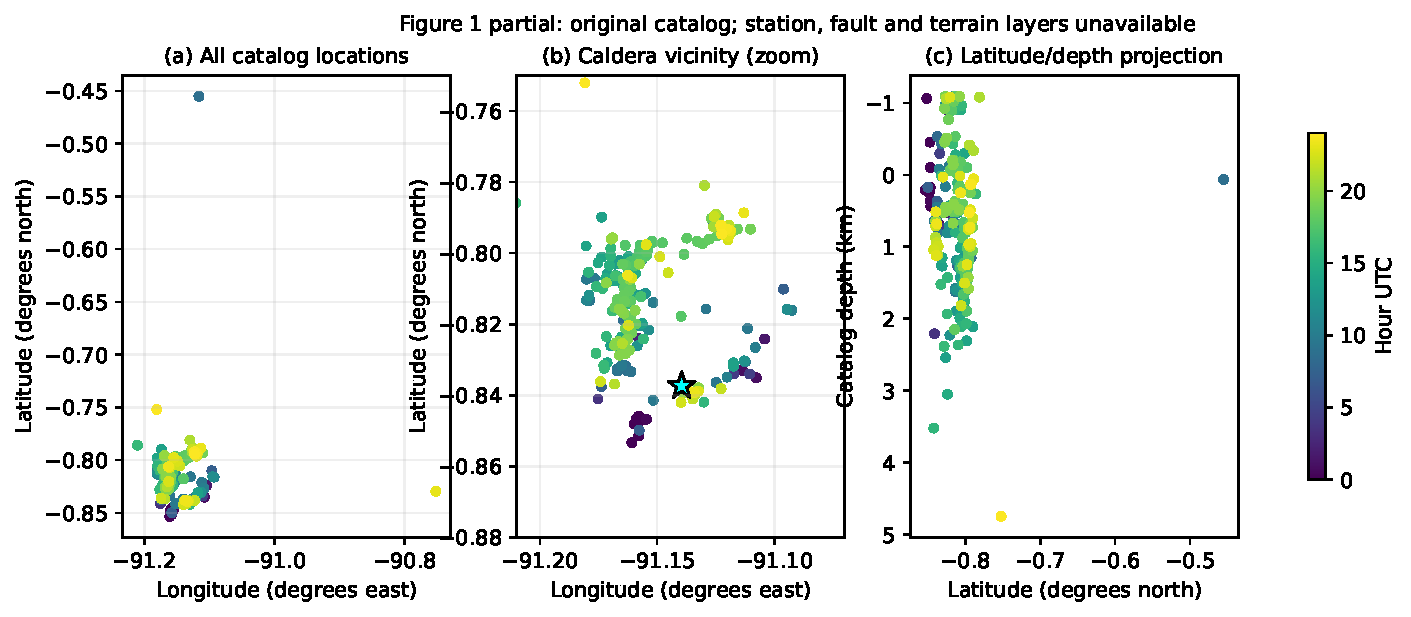
\includegraphics[width=\textwidth]{../results/figures/fig01_original_catalog.pdf}
\caption{Partial reproduction corresponding to main Figure 1. Original Bell archive event coordinates are colored by UTC hour. Panel (a) preserves every catalog location; (b) zooms into the caldera vicinity and marks the maximum-magnitude entry; (c) projects all events onto latitude and source catalog depth. Station layers are supplied separately; this panel lacks fault, terrain and reservoir layers, and the depth datum is unresolved. These are observations from the original catalog, not an enhanced-catalog reconstruction.}
\label{fig:map}\end{figure}
\begin{figure}[p]\centering
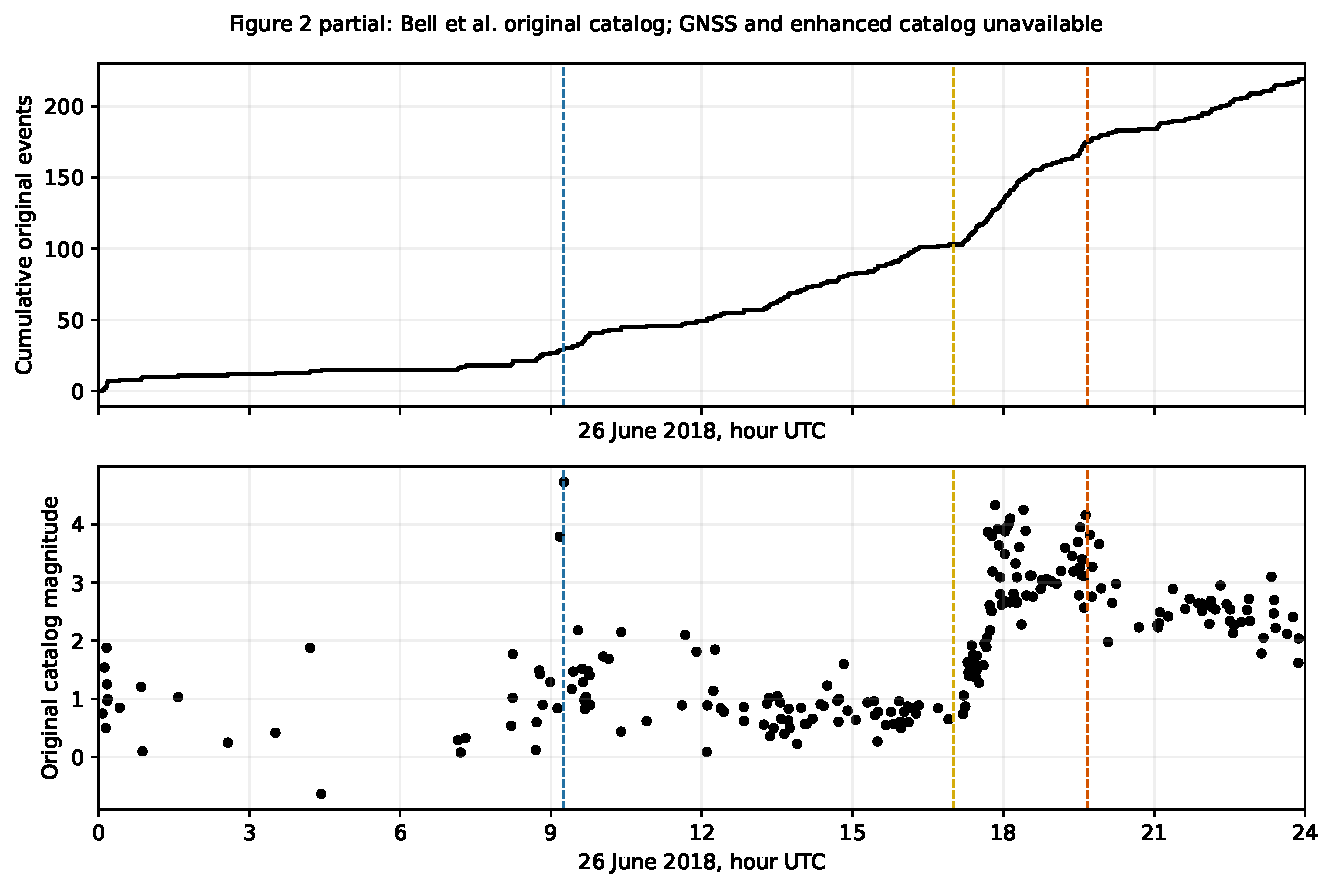
\includegraphics[width=.95\textwidth]{../results/figures/fig02_original_timeline.pdf}
\caption{Partial reproduction corresponding to main Figure 2. Cumulative original events and original catalog magnitudes are plotted against hour UTC on 26 June 2018. Dashed lines give published rounded fault-earthquake, intrusion, and eruption times. Enhanced counts are absent; independent GNSS displacement is supplied separately in Figure~\ref{fig:gnssppp}. The timing lines are literature annotations rather than measurements newly extracted from waveforms or deformation.}
\label{fig:timeline}\end{figure}
\begin{figure}[p]\centering
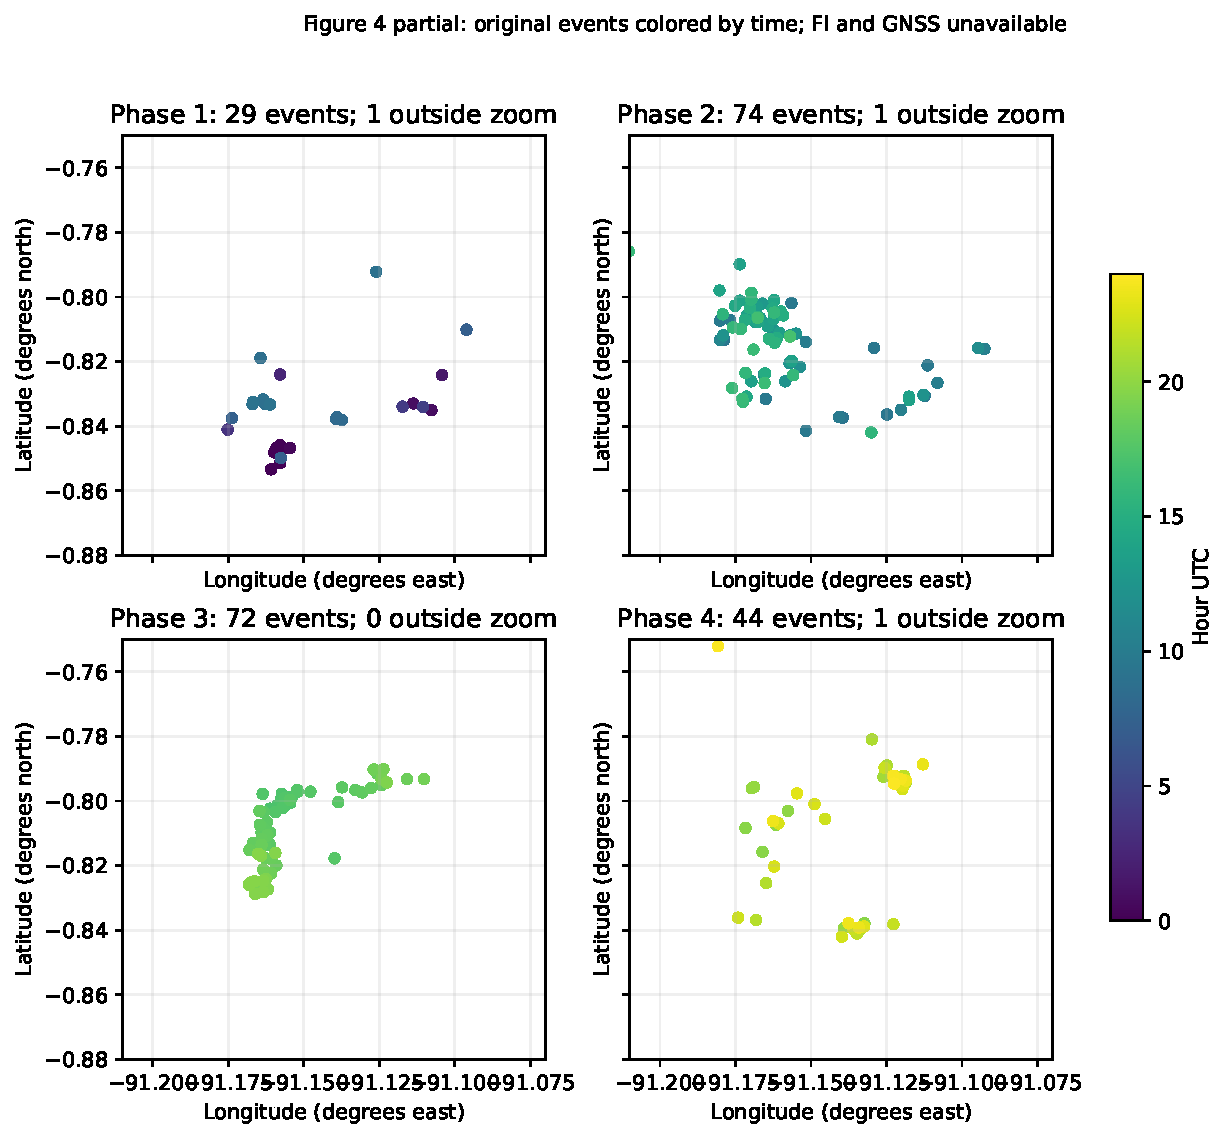
\includegraphics[width=.9\textwidth]{../results/figures/fig04_original_phase_maps.pdf}
\caption{Partial reproduction corresponding to main Figure 4. Each panel plots original event locations in one published phase, with color indicating UTC hour. Titles report full phase counts and locations outside the zoom. GNSS curves are supplied separately in Figure~\ref{fig:gnssppp}; frequency-index color, topography and fault traces are absent from these original-catalog maps. This comparison documents temporal changes in the original catalog without assigning unmeasured LP or VT labels.}
\label{fig:phases}\end{figure}

Twenty-four numerical test cases pass, including GPS-to-UTC conversion, missing RINEX observables, geodetic axis conventions and preservation of solution quality codes. FFT correlation agrees with direct Pearson correlation, and the C++ signed lag kernel agrees with a NumPy reference. Injected positive and negative signals are recovered at their known positions. A constructed Fourier spectrum verifies the amplitude-based FI boundary. Additional tests check transitive components, magnitude conversion, recurrence pairing, regression and jackknife calculations, arrival-window boundaries, and geodetic differencing. A synthetic end-to-end window-CLI test verifies classification, family membership and interval output. A further overlap test verifies probability averaging, blind edges and refusal of incomplete three-component inputs. Constructed test signals are algorithm validation data and are excluded from observational products.


\begin{figure}[p]\centering
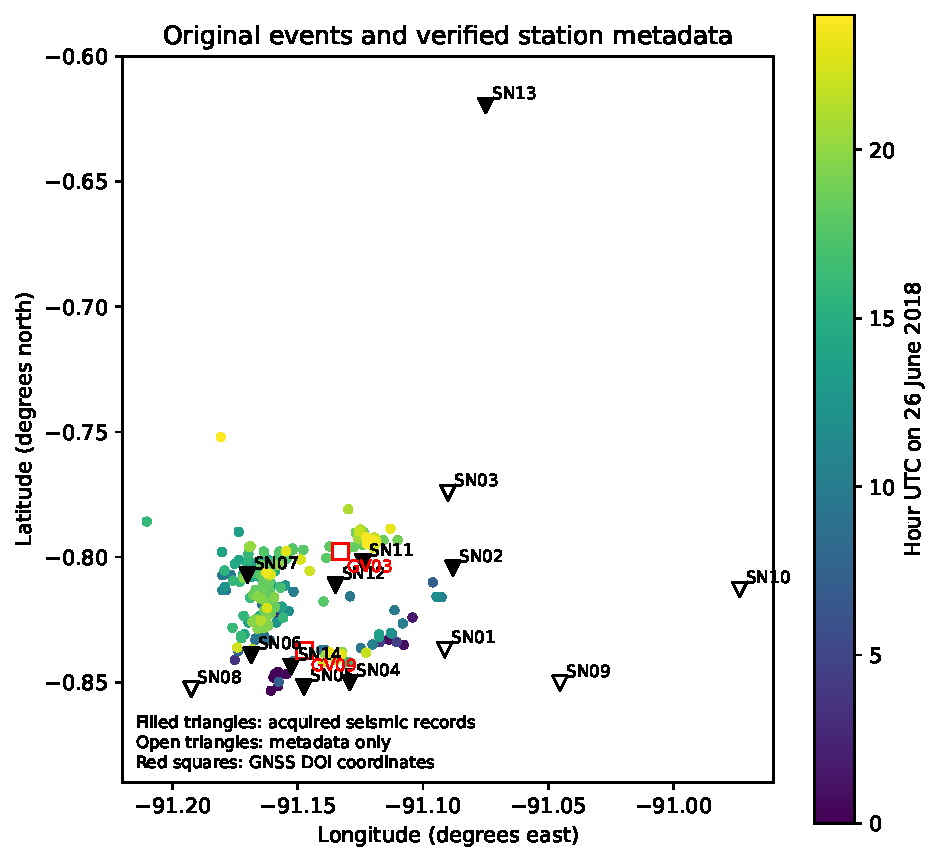
\includegraphics[width=.75\textwidth]{../results/figures/fig01_all_stations.pdf}
\caption{Additional reconstruction of station distribution for main Figure 1. Triangles show fourteen archived 8G/EC seismic metadata stations. Filled triangles mark the nine stations with acquired waveforms; open triangles mark metadata-only stations. Red squares give rounded GV03/GV09 coordinates from DOI landing pages; their coordinate datum is not independently verified. Original-catalog events are colored by UTC hour. Terrain and faults remain absent. Metadata presence is not evidence of recording availability.}
\label{fig:stations}\end{figure}

\subsection{Candidate phase-picking execution}
We execute the public Volpick checkpoint on all 168 acquired 8G station-hours, obtaining 6,908 candidate P picks and 6,379 candidate S picks. The supplement reports 13,144 P and 12,196 S candidates before association across its study network; our differences are therefore $-6,236$ and $-5,817$, respectively. Seven-station coverage and independently specified processing/checkpoint details prevent interpreting these differences as event completeness. The published 6,261 P and 5,159 S main-text arrivals instead refer to associated arrivals, so they are a different comparison target.

The asynchronous SeisBench stream wrapper stalled in this environment. Direct execution uses the checkpoint's own batch preprocessing, forward and postprocessing methods, with averaged finite overlapping probabilities. We use 60-second windows at 50\% overlap, a four-corner causal 2--12 Hz filter, per-window pretrained-model normalization, five-second edge blinding and the package's probability-trigger routine at 0.2. Filter order/phase, normalization, blinding, stacking and exact checkpoint equivalence are not established as the original implementation. Checkpoint hashes, model settings and per-hour execution records are saved. No false-pick rate, event completeness or new hypocenter is inferred from these candidate arrivals.

\begin{figure}[p]\centering
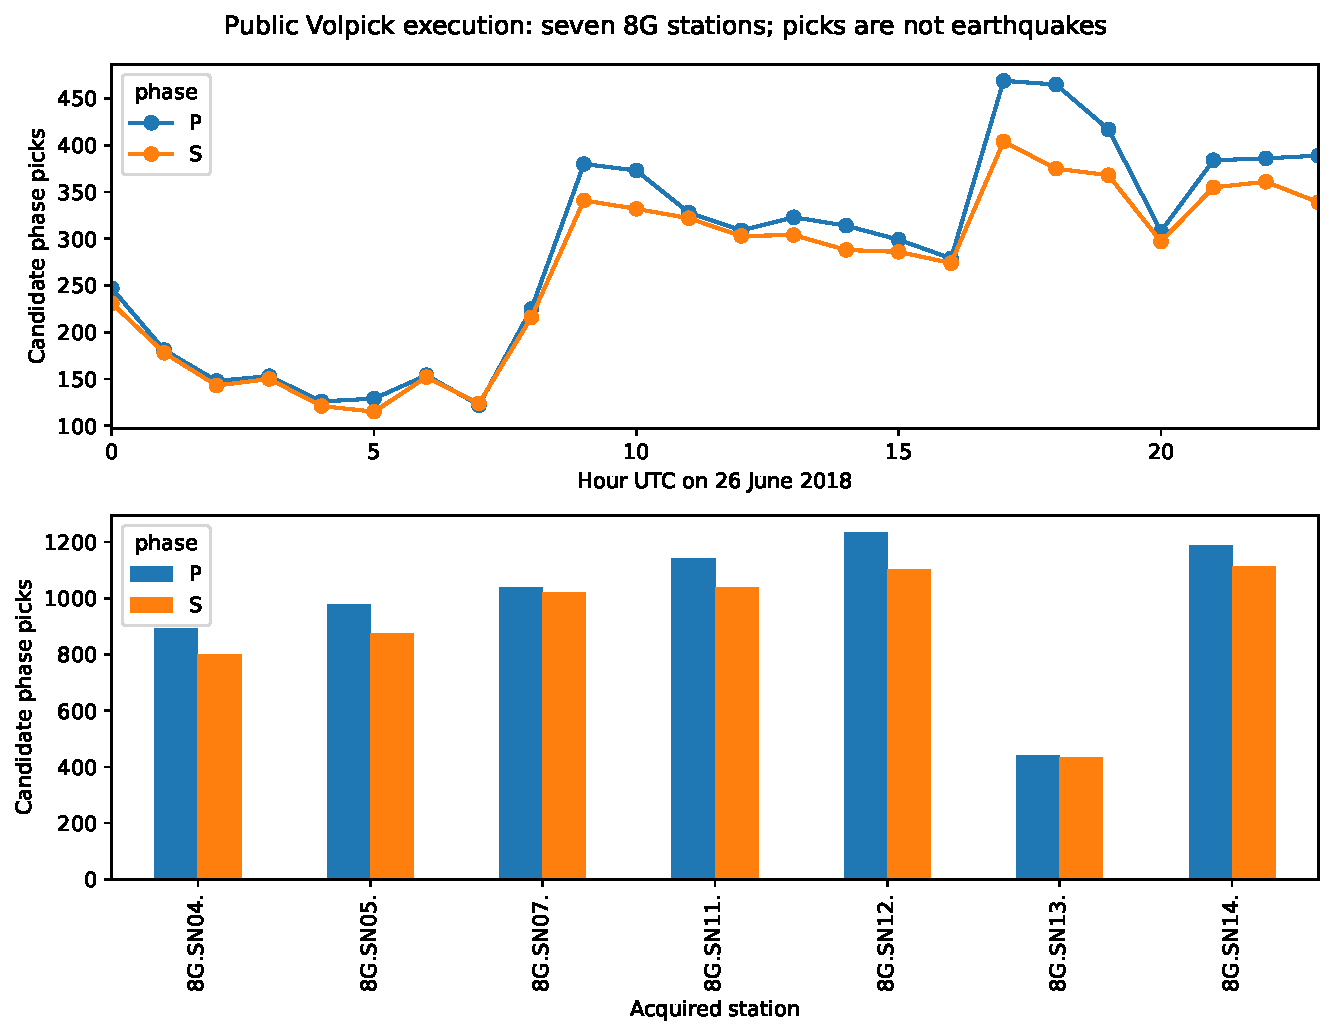
\includegraphics[width=.9\textwidth]{../results/figures/phase_pick_counts.pdf}
\caption{Candidate phase picks from the completed public-model execution on seven acquired 8G stations. Upper panel counts candidates by UTC hour; lower panel counts them by station. P and S denote model-assigned phase labels, not independently validated event arrivals. Differences in station coverage, noise and model response affect the distributions. This diagnostic is not a reproduction of the enhanced earthquake count curve.}
\label{fig:picks}\end{figure}

\subsection{Independent reproduction of PAYG day plots}
We obtain four full-day IU.PAYG.00.BHZ records corresponding to Supplementary Figure 5. We remove the epoch instrument response to recover velocity in m/s, using a 0.01, 0.02, 8, 9 Hz stabilization prefilter and no water level. These are independent processing choices because the original stabilization settings are unspecified. Each contiguous segment is processed separately; gaps are not interpolated. Thirty-minute rows use one-second minimum/maximum envelopes. Per-day display gain is the 99th percentile of absolute velocity, with no amplitude clipping. Major wave packets occur in the corresponding published time rows, but identical amplitudes cannot be claimed without matching preprocessing and gain.

\begin{figure}[p]\centering
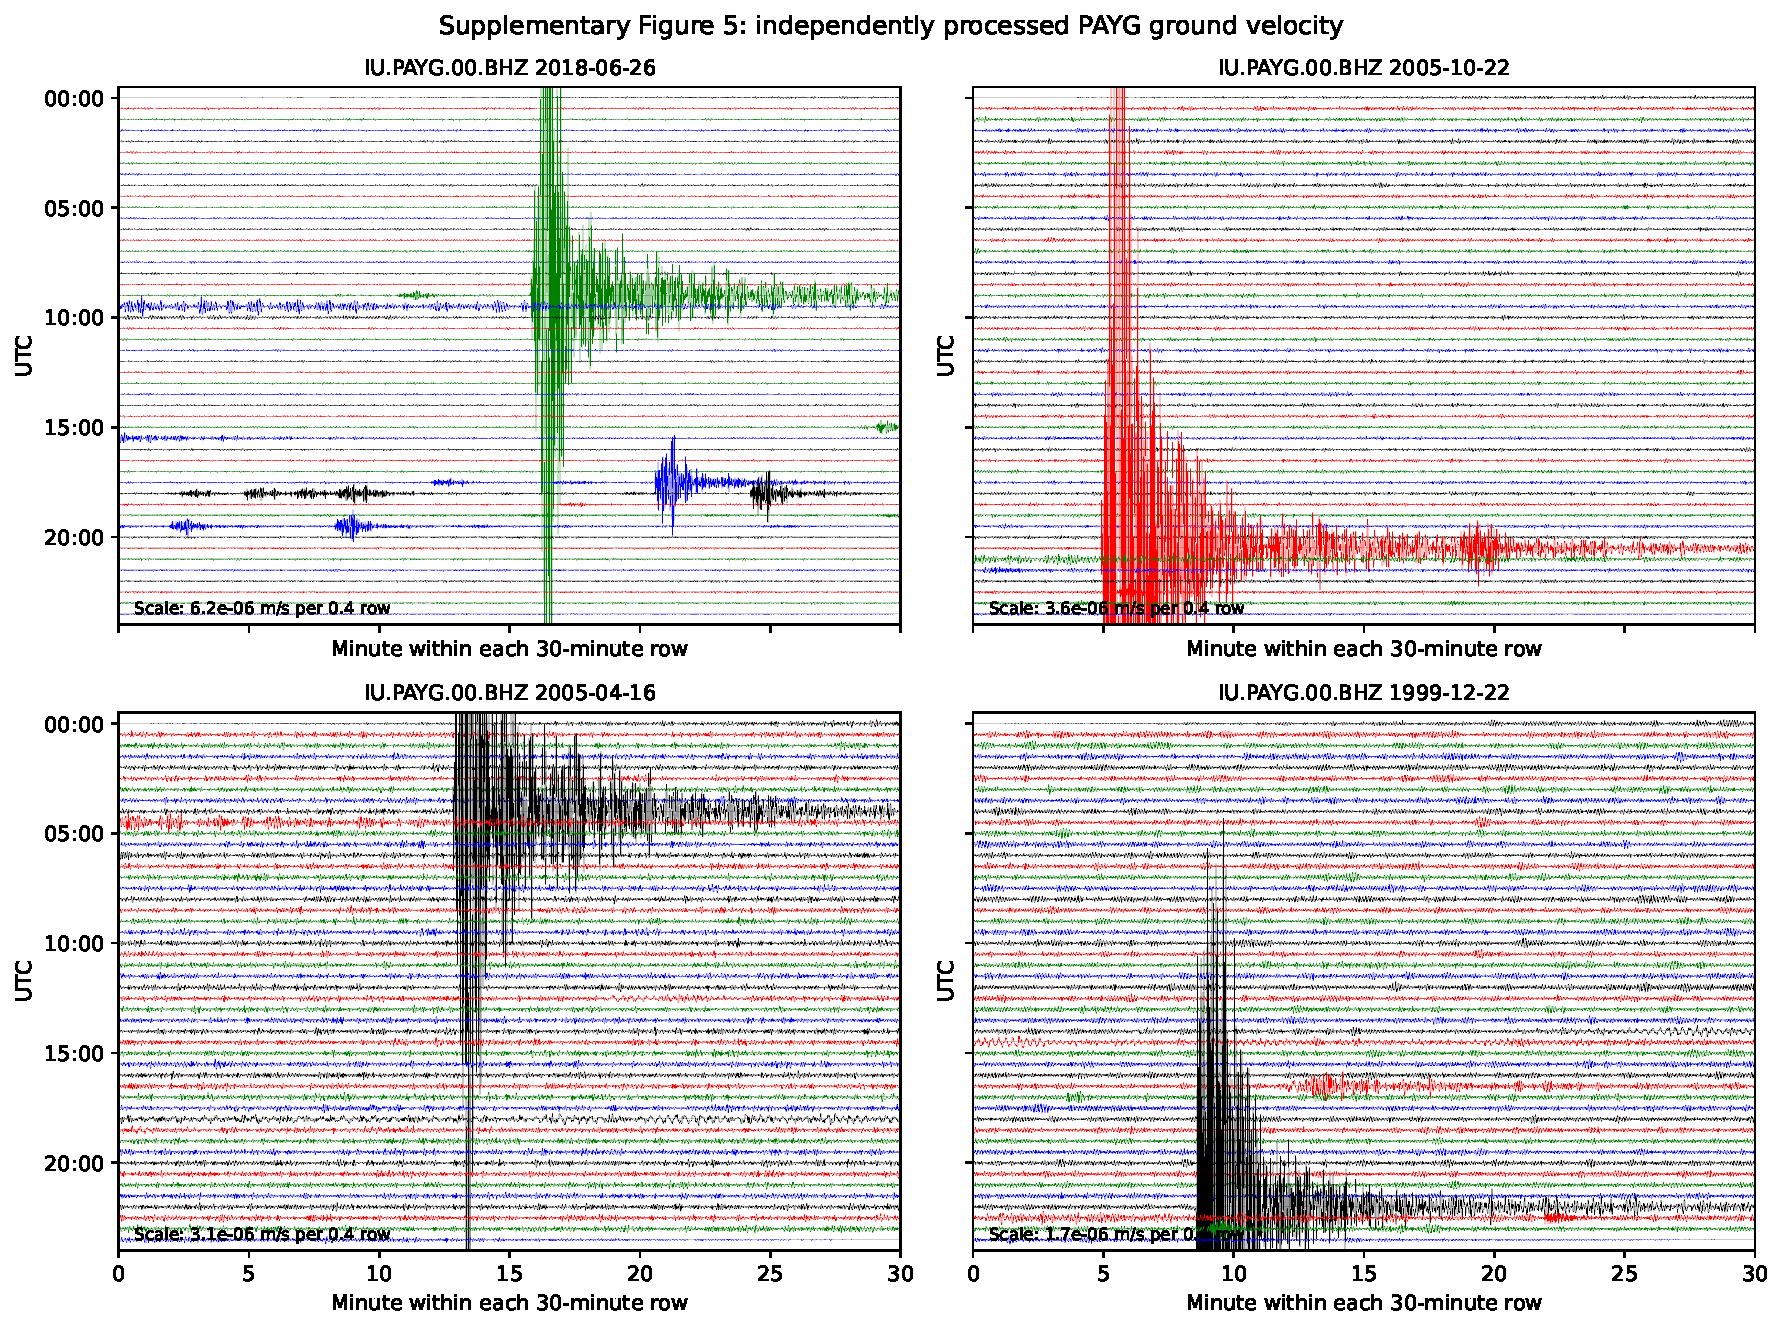
\includegraphics[width=\textwidth]{../results/figures/figS05_payg_dayplots.pdf}
\caption{Independent computational reproduction of Supplementary Figure 5 from raw PAYG vertical records and instrument responses. Panels cover 26 June 2018, 22 October 2005, 16 April 2005 and 22 December 1999. All four records span a complete day. Color cycles across thirty-minute rows; ordinate labels indicate UTC and the abscissa gives minutes within each row. Insets state the separate velocity display scales. Response stabilization and display gain are independent documented choices, so this comparison tests timing and morphology rather than exact amplitude agreement.}
\label{fig:payg}\end{figure}


\subsection{Independent high-rate GNSS analysis}
We decompress Hatanaka records and validate unique chronological epoch/satellite observations and finite dual-frequency measurements. RINEX GPS epochs are converted to UTC with an 18-second offset. GV03 has nine internal gaps; its longest contains both one-hour windows around the fault earthquake. GV09 has complete observation coverage. VCH1 waveform acquisition is skipped at the user's instruction and remains a coverage limitation.

Independent RTKLIB 2.4.2 processing \citep{rtklib} uses ESA final reprocessed five-minute orbits, 30-second clocks and IGS20 antenna calibrations. Station-specific broadcast navigation is required; GV03 navigation alone would omit GV09 solutions during the GV03 outage. Settings include forward GPS-only float-ambiguity kinematic PPP, ionosphere-free dual-frequency observations, a 15-degree elevation mask, estimated zenith tropospheric delay and solid Earth tides. This differs from the paper's GIPSY-OASIS II, VMF1 and FES2004 processing. Ocean loading is not applied, and the downloaded current antenna calibration is not asserted to match the historical ESA revision. Settings and product hashes are machine-readable and retained.

We rotate ECEF positions to east/north/up axes at each header coordinate. A conservative independent screen requires PPP quality code 6, at least five satellites and one hour since initialization or a gap longer than five minutes. Changes use the 01:00--02:00 UTC mean as a datum. Of 2,880 GV09 and 1,431 GV03 solution epochs, 2,760 and 836 pass this screen. Screening is not proof of convergence or absolute position accuracy.

At the catalog earthquake time 09:15:32.299 UTC, one-hour post-minus-pre means at GV09 give east $-0.09460$ m, north $+0.84616$ m and up $+1.86707$ m, with 120 epochs in each window. Vertical within-window standard deviations are 0.00788 and 0.02528 m. These describe scatter and evolving deformation, not confidence limits. Song et al. report at least 1.83 m uplift, a lower bound rather than an exact target. The computed change exceeds that bound by 0.03707 m and is consistent with its scale. Different corrections and postseismic contributions preclude a stronger numerical agreement claim. GV03 has no coseismic estimate because observations are absent.

\begin{figure}[p]\centering
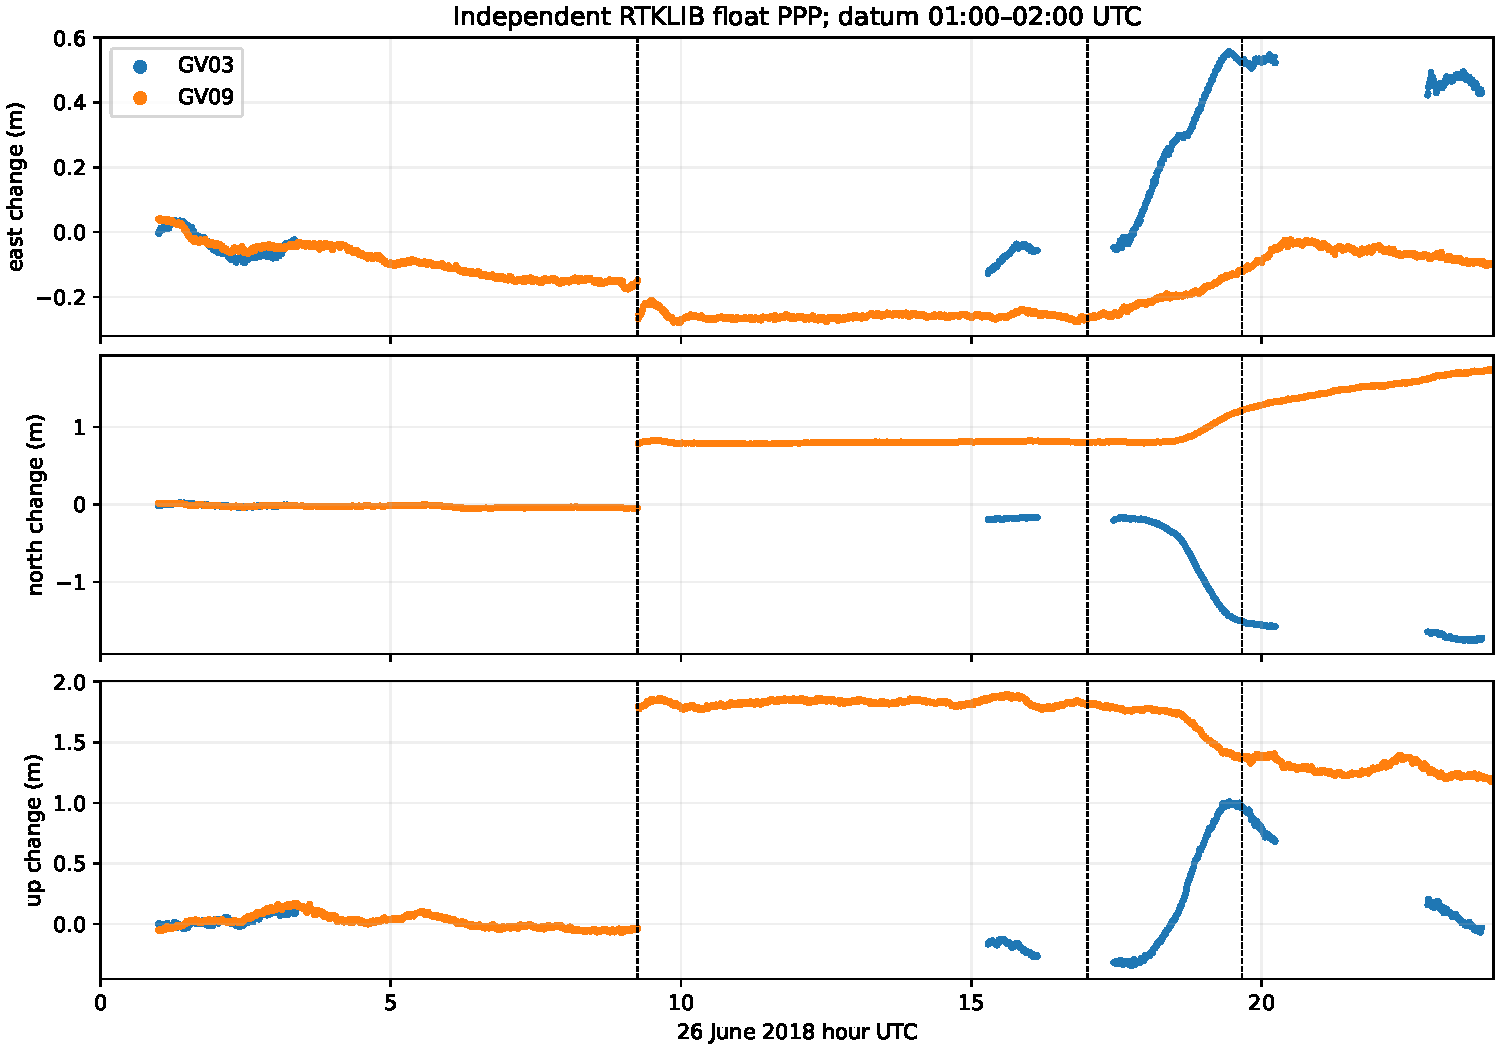
\includegraphics[width=\textwidth]{../results/figures/gnss_independent_ppp.pdf}
\caption{Independent high-rate PPP positions for GV03 and GV09. Points pass the stated quality and post-gap screen. Datum is the 01:00--02:00 UTC mean; coordinates are east, north and up. No gaps are interpolated. Dashed lines annotate published rounded fault-earthquake, intrusion and eruption times; an onset time is not independently fitted. Software, tropospheric corrections and loading differ from the published analysis.}
\label{fig:gnssppp}\end{figure}

A second calculation provides a relative-baseline cross-check. Combined forward/backward dual-frequency kinematic processing uses broadcast ephemerides, a 15-degree mask and continuous ambiguity resolution with ratio threshold 3. The computational GV03 reference coordinate is fixed, although that station physically moves. We require simultaneous observations, zero reference age and relative quality codes 1 or 2, rejecting single-point positions. Of 2,140 output epochs, 1,410 remain: 1,363 fixed and 47 float. Fixed ambiguities are a quality indicator rather than proof against false fixes. On 814 common screened epochs, PPP-derived and relative baselines, projected in the same axes and aligned over 01:00--01:30 UTC, differ by RMS 0.0317 m east, 0.0162 m north and 0.0647 m up. Shared observation errors are correlated; this is a processing consistency check rather than independent validation. The datum is 00:30--01:30 UTC; no relative coseismic estimate is possible. Later changes constrain motion between stations, not absolute motion of either station.

\begin{figure}[p]\centering
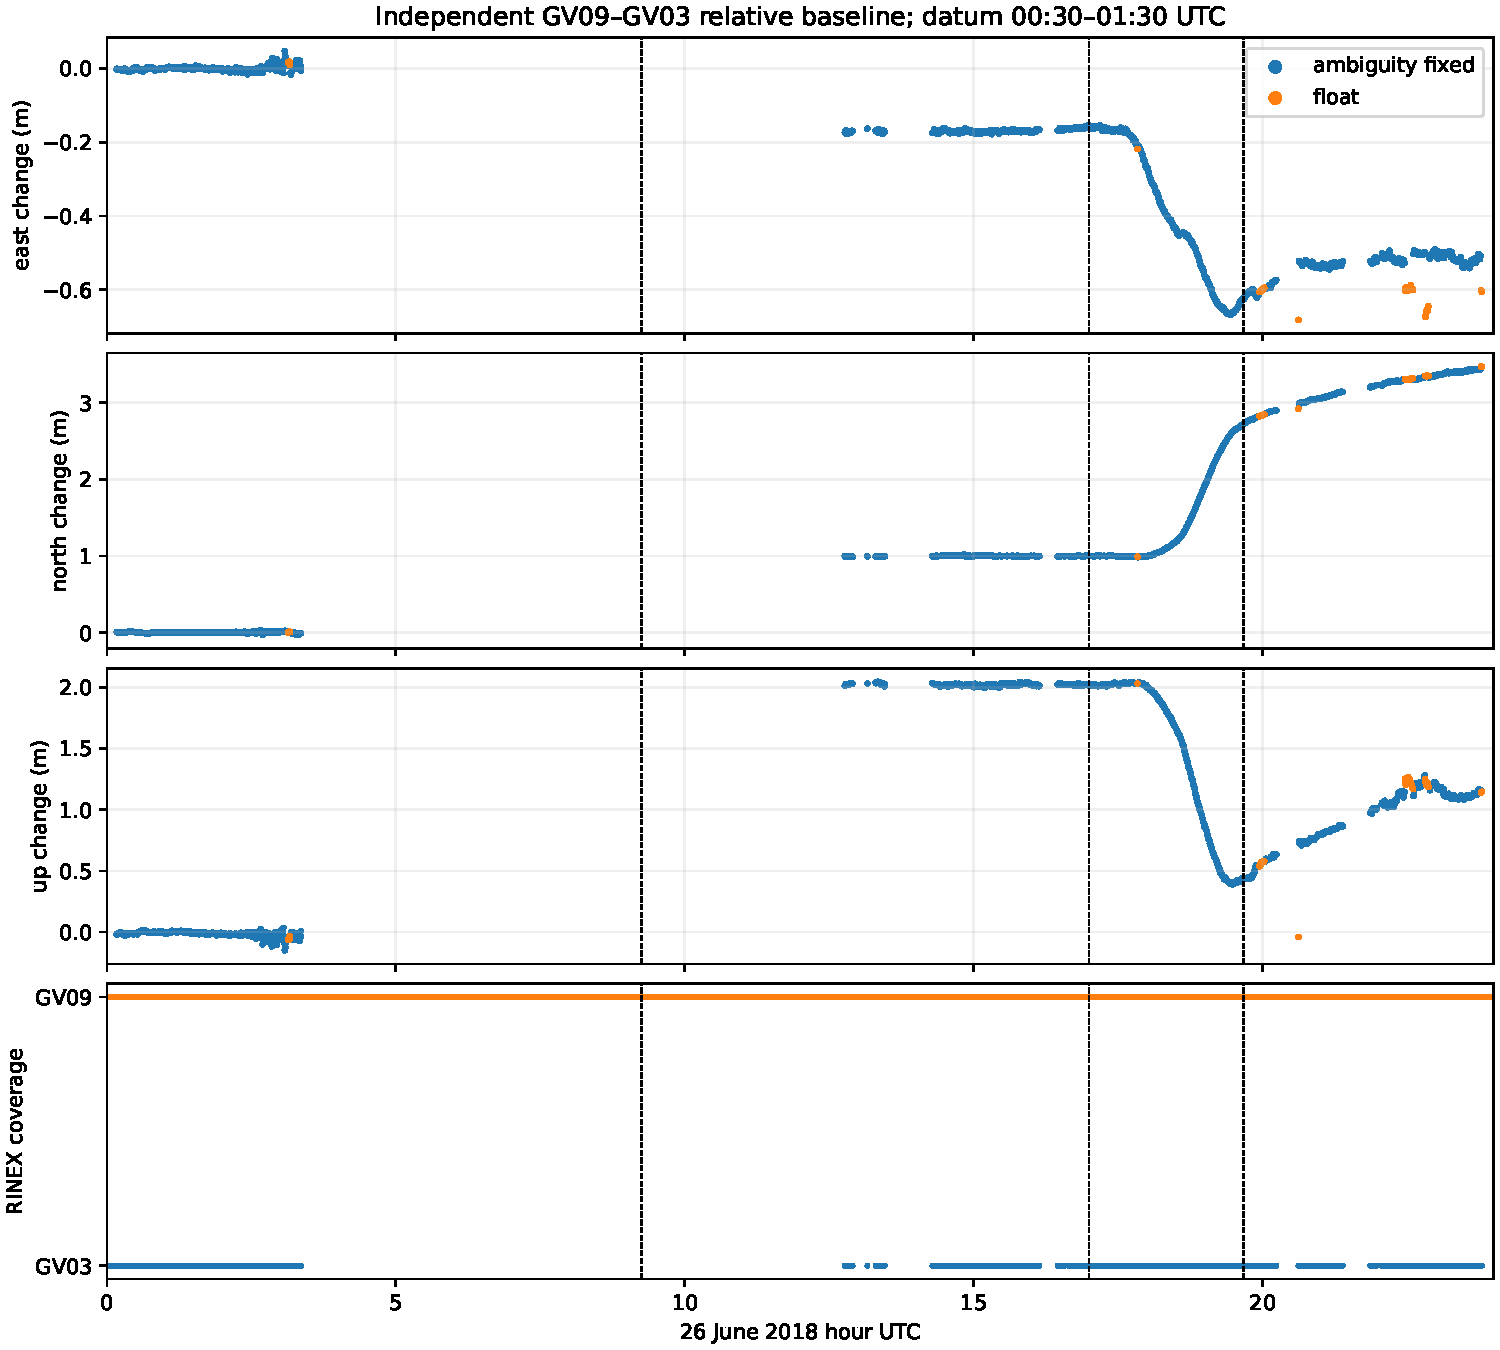
\includegraphics[width=.9\textwidth]{../results/figures/gnss_relative_baseline.pdf}
\caption{Independent GV09--GV03 relative baseline and raw observation coverage. Blue and orange points distinguish fixed and float relative ambiguities. Missing or stale-reference solutions are excluded. Both stations may move; the ordinate is relative baseline change. The long GV03 outage prevents a fault-earthquake displacement measurement.}
\label{fig:gnssrelative}\end{figure}

\subsection{Published 1-D location approximation}
We adopt numerical P and S values from Tepp et al. (2014), Table 1, Model F \citep{tepp2014}. Original nodes at 0, 2, 4, 8, 12, 20 and 40 km below sea level are combined with the published top grid value at $-2$ km (3.95/2.19 km/s). Piecewise-linear interpolation and PyOcto surface elevation correction at 4.29/2.38 km/s are declared approximations. They are not the target paper's model, and no new Vp/Vs is invented.

The declared search domain is latitude $-0.90$ to $-0.76$, longitude $-91.22$ to $-91.08$, and depth 0--30 km below sea level. Travel-time tables use 0.1-km spacing; location nodes use 1 km. Association requires at least four P and one S arrival with 0.5-s match tolerance and 2-s minimum interevent time. Domain center and other PyOcto defaults are independent choices. Only the seven already-picked 8G stations enter the approximation. Computational time slices are 300 s with 16 workers; these are declared independent settings. Above-sea-level sources are excluded by the 1-D implementation. HypoInverse remains unexecuted and an independent catalog-time-only HypoDD pilot is evaluated separately; candidate associations cannot be equated to the published 694 relocated or 1,935 enhanced events.


The nominal run produces 536 candidates with 2,730 P and 2,408 S assigned arrivals. Median absolute residual is 0.09821 s and the maximum is 0.49953 s. Validation verifies phase requirements, residual limits, unique station/phase assignments and domain bounds. A final returned-residual gate enforces the 0.5-s tolerance after PyOcto refinement, followed by rechecking phase minimums. No nominal arrivals are removed. Candidate origin times are within two seconds of 199 distinct original entries, but time proximity does not establish event identity or completeness. Unmatched candidates are not automatically new earthquakes. Approximately 53.9\% occupy the shallowest 0.46875-km location node; coarse nodes and the excluded above-sea-level domain limit depth interpretation.

Uniform P and S speed perturbations of $-5\%$ and $+5\%$ produce 536 and 534 candidates after final quality control. Mutual nearest time matches within two seconds give 531 and 530 correspondences. Median horizontal and depth shifts are zero at this coarse grid; 90th-percentile shifts are about 1.373 km horizontally and 0.938 km in depth. These are declared sensitivity cases rather than confidence bounds. Grid quantization limits the meaning of unchanged median locations.

\begin{figure}[p]\centering
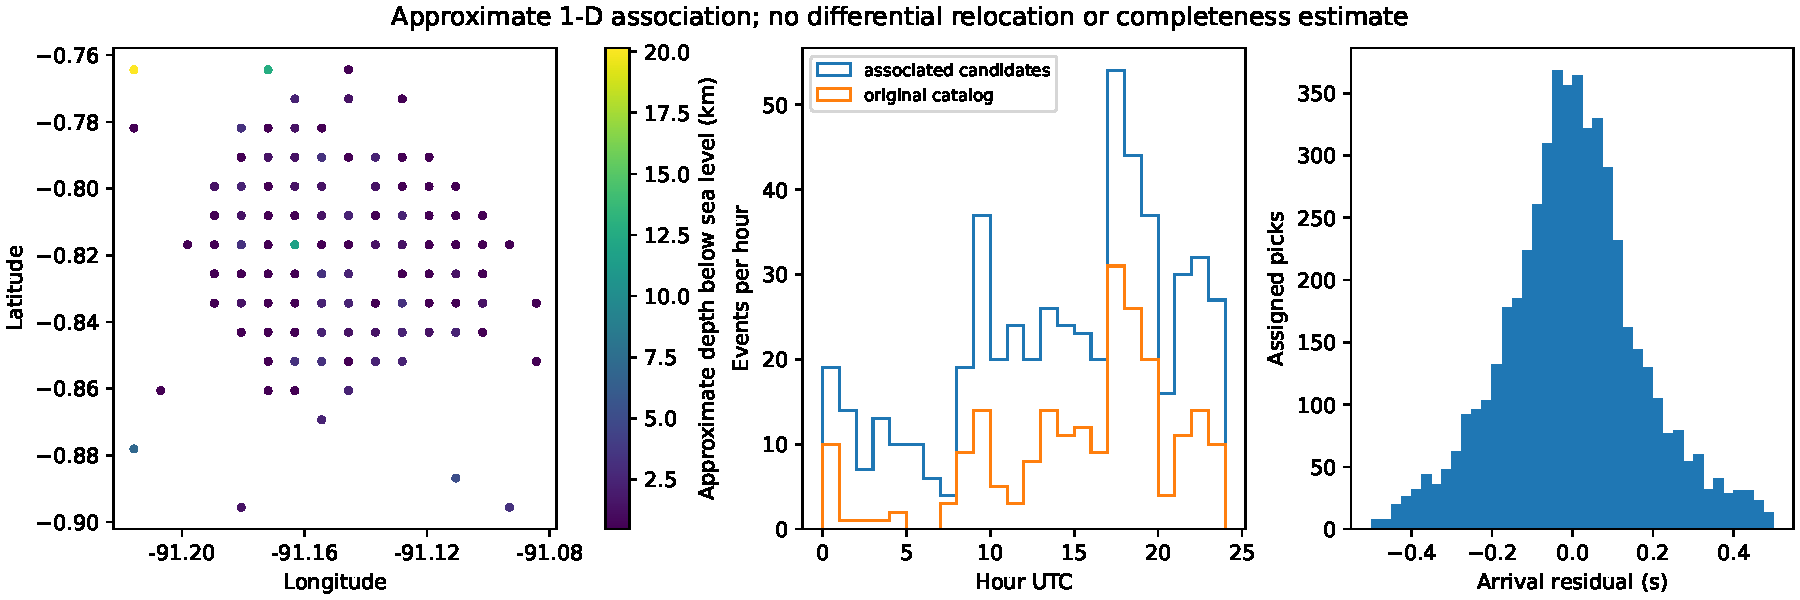
\includegraphics[width=\textwidth]{../results/figures/approximate_association.pdf}
\caption{Approximate candidate earthquake locations, hourly counts and arrival residuals. Published Tepp Model F velocities replace the original study model. Counts are compared with the original catalog rather than labeled as the enhanced population. No differential relocation, magnitude estimation or false-detection assessment has been performed. The shallowest depth-node concentration is a resolution limitation.}
\label{fig:association}\end{figure}


\subsection{Observed spectral classification and template expansion}
Assigned P/Z and S/horizontal windows are extracted from real 64-s contexts. Instrument response is removed to velocity with a 0.5, 1, 22, 24 Hz stabilization taper and no water level. A four-corner zero-phase 2--20 Hz filter precedes 50-Hz resampling. Signal windows span $[-1,4]$ s relative to arrivals, with RMS noise measured over $[-11,-6]$ s. An alternate $[-6,-1]$ s noise window tests this independent choice. Sixty-three 64-versus-128-s context comparisons give minimum NCC 0.9999999999999714 and maximum FI shift $3.20\times10^{-9}$. These examples constrain context sensitivity without establishing all waveform quality.

Using P/Z windows with SNR at least two, the seven-station candidates contain 96 LP, 438 VT and two unclassified events. The signed pair kernel searches $\pm0.2$ s. Component coefficients are averaged within station and stations receive equal weight. With four common stations, edges above 0.7 and components of at least ten events, one ten-event LP family occurs from 14:21:48 to 16:54:32 UTC. Its mean recurrence is 1018.18 s and mean/std periodicity is 1.19869 with population standard deviation, or 1.13014 with sample standard deviation. Zero-lag analysis finds no qualifying families; a one-common-station screen yields a 17-member family. Therefore, station and lag choices affect membership.

Full-day matching uses 447 SNR-qualified templates on real 30-s-padded hourly blocks. The positive network threshold is $\max[9\,\mathrm{median}(|\mathrm{NCC}|),0.4]$. All 447 templates recover themselves, with minimum self-NCC 0.71785 and maximum timing discrepancy 0.01779 s. After declared two-second suppression and exclusion around all 536 associated candidates, 1,007 additional detections remain. The 1,543-event population has inherited labels of 453 LP, 1,088 VT and two unclassified events. Template locations are approximate and inherited, not independently relocated. Additional detections have directly measurable FI in 646 cases; 520 agree with inherited type, while 361 lack qualifying P/Z spectra. Correlation alone does not quantify false detections.

The two EC stations add 1,665 P and 1,622 S picks, giving nine-station totals of 8,573 P and 8,001 S. Gap-free three-component segments are processed without interpolation. The nine-station association yields 716 candidates, with 7,531 assigned arrivals. This is a separate coverage experiment; it is not silently merged with seven-station template locations. The count difference demonstrates coverage sensitivity, not agreement with the source 694 relocated events.

\begin{figure}[p]\centering
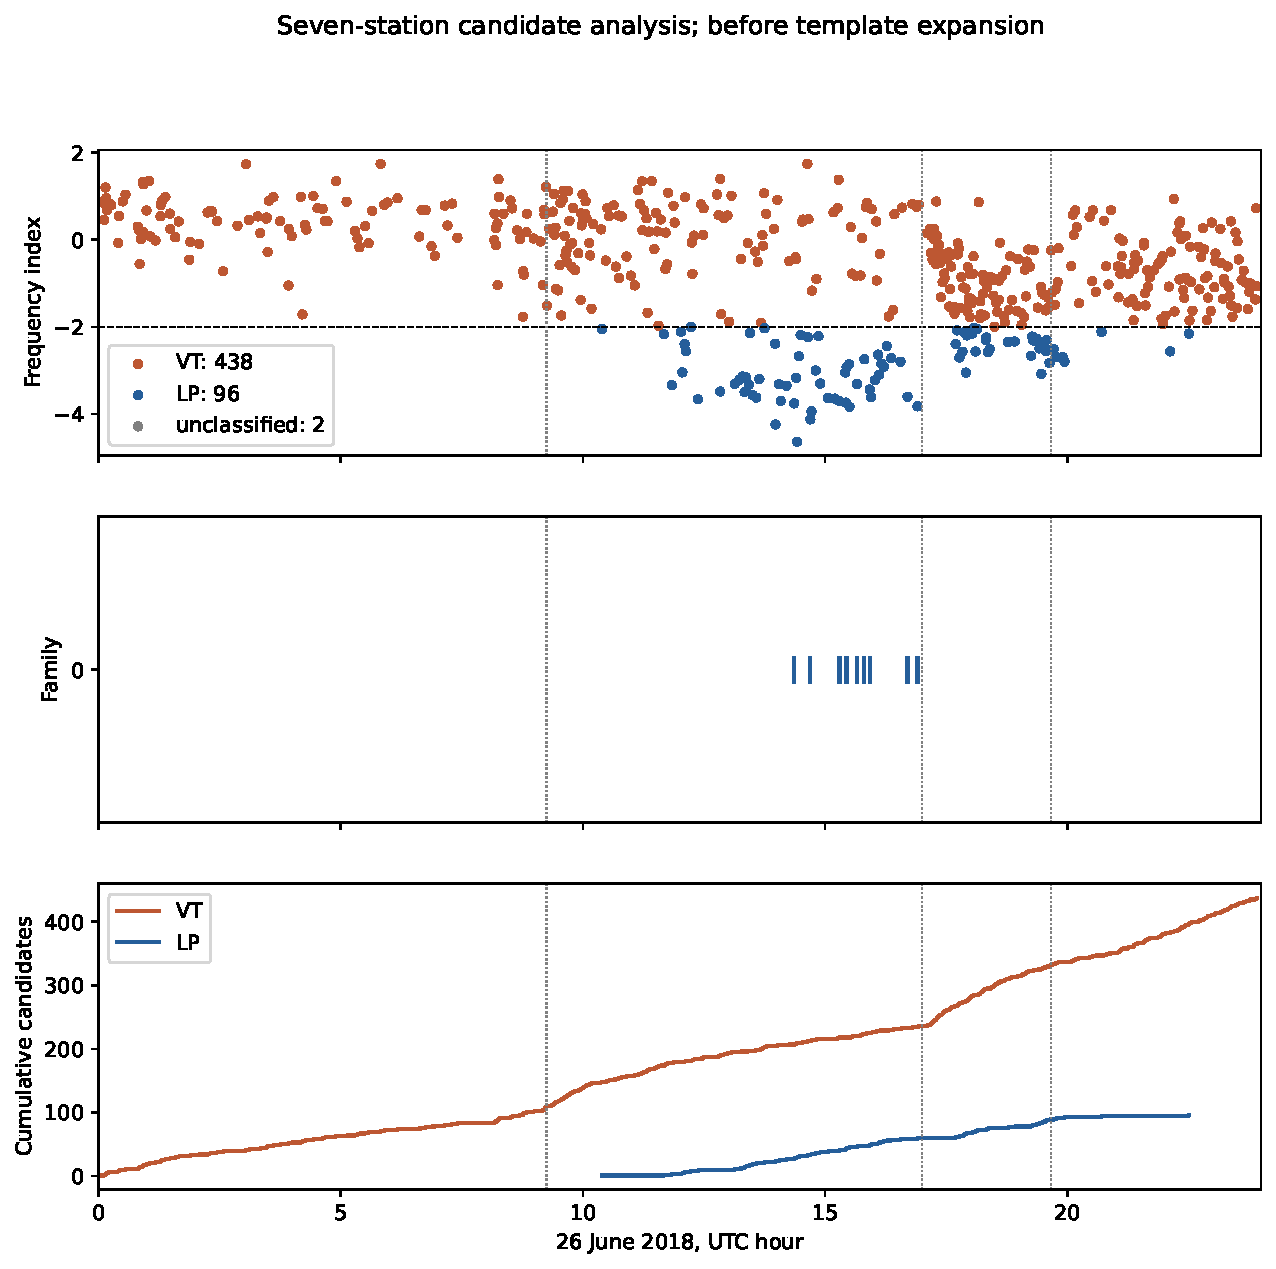
\includegraphics[width=.95\textwidth]{../results/figures/candidate_frequency_families.pdf}
\caption{Independent counterpart of main Figure 3 before template expansion. FI uses response-corrected P/Z windows; the dashed threshold is $-2$. The family raster shows the ten-event connected component under the declared lag and station screen. Vertical lines show published phase boundaries. Counts describe approximate candidates, not the source catalog.}\label{fig:candidatefi}\end{figure}

\subsection{Approximate magnitudes and moment estimates}
Actual horizontal data are response-corrected on 64-s contexts before Wood--Anderson simulation; no additional 2--20 Hz bandpass is applied to magnitude waveforms. The simulation uses the ObsPy one-zero velocity-input response \citep{obspywa}, poles $-6.283\pm4.7124i$ rad/s and sensitivity 2080. The mean two-horizontal-component peak-to-peak amplitude is converted to millimetres in $[-1,4]$ s S-arrival windows. Both components must pass the independent SNR screen. With approximate epicentral distance $R$ in kilometres, the supplementary Bakun--Joyner equation gives station ML; the event value is the station median. We obtain 528 template-candidate magnitude estimates.

Additional-event amplitude ratios use the dominant eigenvector slope of the centred template/detection waveform covariance, after best signed lag alignment on SNR-qualified P/Z windows. Positive NCC and positive ratios are required. The published relative expression $M_{L,d}=M_{L,t}+0.7\log_{10}\alpha$ is applied, but the PCA formulation is independent because the source implementation is unavailable. In total 1,154 candidates have approximate magnitude estimates. The published empirical conversion supplies moment rather than a spectral source inversion. The source Wood--Anderson sensitivity and amplitude units are not explicit: changing sensitivity from 2080 to 2800 shifts ML by 0.12910, while using the standard half-peak-to-peak convention \citep{hutton1987} shifts ML by $-0.30103$. These are convention sensitivities, not estimated confidence bounds.

Five enhanced negative network pairs qualify for review; three baseline pairs have polarity-preserving station overlay plots. Different lags and narrow-band phase shifts prevent equating these with confirmed source reversals. No source mechanism is inferred from a negative coefficient alone.


\subsection{Expanded families and recurrence sensitivity}
The four-common-station graph yields two LP families with 12 and 11 members, totalling 23 events. The first begins at 11:20:13 UTC, approximately two hours after the fault earthquake. Its mean recurrence is 1454.55 s and population periodicity 1.23817; the second has mean recurrence 916.36 s and periodicity 1.07792. This screen finds no VT family with at least ten members. The source reports 29 families with 714 members, so its population is not reproduced. A permissive one-common-station screen instead yields 14 families with 452 members. Zero-lag and noise-window experiments change these counts. This sensitivity prevents interpreting the primary count deficit as missing physical families alone.

For the strict LP families, 21 preceding-interval pairs give OLS slope $-0.02548$, intercept 11.35680 and $R^2=0.002715$ in log--log space. The one-station sensitivity supplies 129 LP pairs before 17:00 UTC and 175 VT pairs after that boundary. Their OLS slopes are 0.05278 and 0.50334, with $R^2=0.007338$ and 0.148292. Following-interval pairing gives slopes $-0.04993$ and 0.48241, respectively. These weak LP and positive VT OLS relationships qualitatively resemble the reported contrast, but do not reproduce its regression statistics.

Independent RANSAC uses two-point minimal samples, 1000 trials, seed 20261009 and the estimator's default residual threshold, the MAD of log moment. In the permissive preceding-pair case, LP and VT slopes are 0.07646 and $-0.04912$. All-point $R^2$ is $-0.04489$ and $-0.18019$, while inlier $R^2$ is 0.16623 and 0.02706. Negative all-point $R^2$ means these robust fits predict the complete population worse than its mean. The source's unspecified inlier and estimator conventions prevent a direct equality test. We retain all-point and inlier statistics separately rather than selecting the more favourable value.

Increasing the matching NCC floor from 0.4 to 0.5, 0.6 and 0.7 reduces additional candidates from 1007 to 534, 276 and 112. Increasing the MAD multiplier from nine to 15 at a 0.4 floor gives 881 candidates. These are threshold sensitivities, not a calibrated false-positive rate. A full-day waveform-shape control uses ten LP and ten VT templates whose individual amplitude spectra are preserved while channel phases are independently randomized (seed 20261009). The same network thresholds yield zero raw control peaks. The smaller control library and destroyed channel coherence preclude scaling this result into an earthquake false-positive rate. The earliest inherited LP detection at 10:05:51 has direct FI $-0.98968$ on one qualifying station and is therefore VT by that direct measurement. Inherited labels alone cannot establish the onset of LP activity.

\begin{figure}[p]\centering
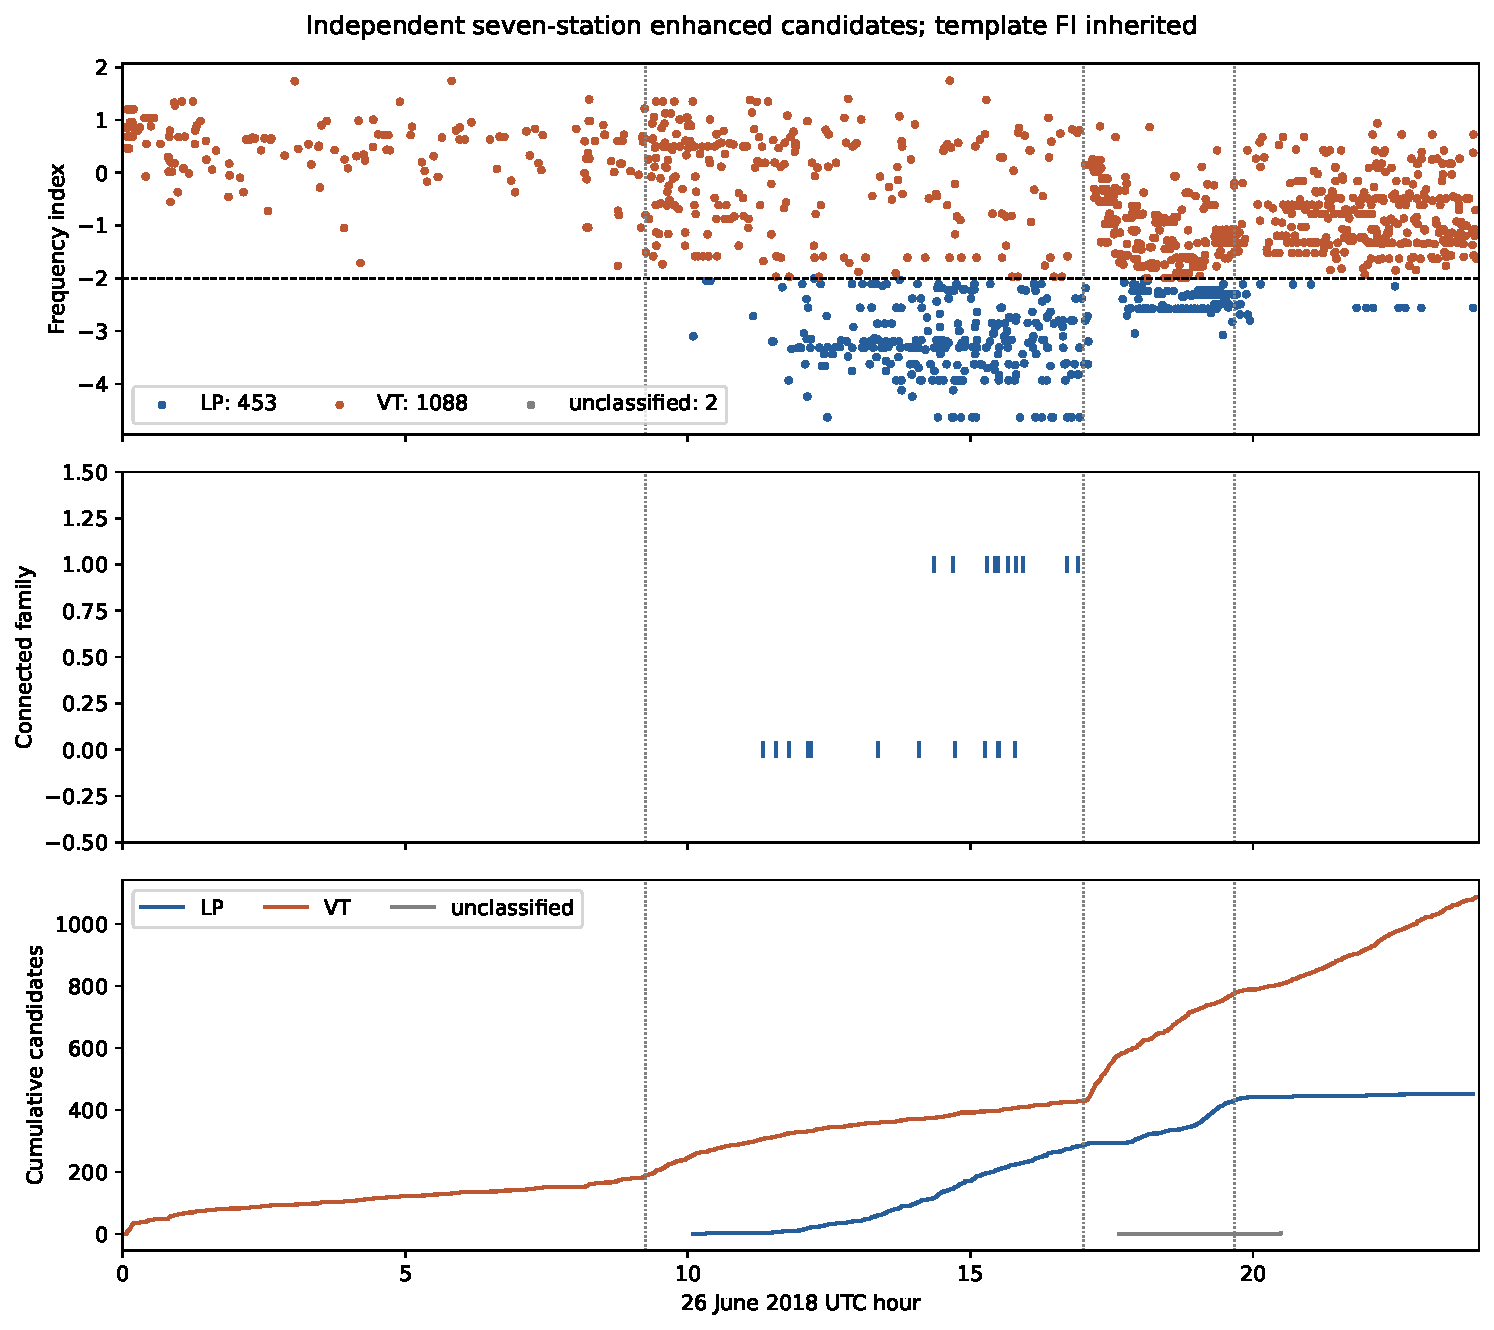
\includegraphics[width=.95\textwidth]{../results/figures/enhanced_frequency_families.pdf}
\caption{Independent enhanced counterpart of main Figure 3. The primary graph contains two LP families; additional detections inherit template FI. The population differs from the published enhanced catalog.}\label{fig:enhancedfi}\end{figure}
\begin{figure}[p]\centering
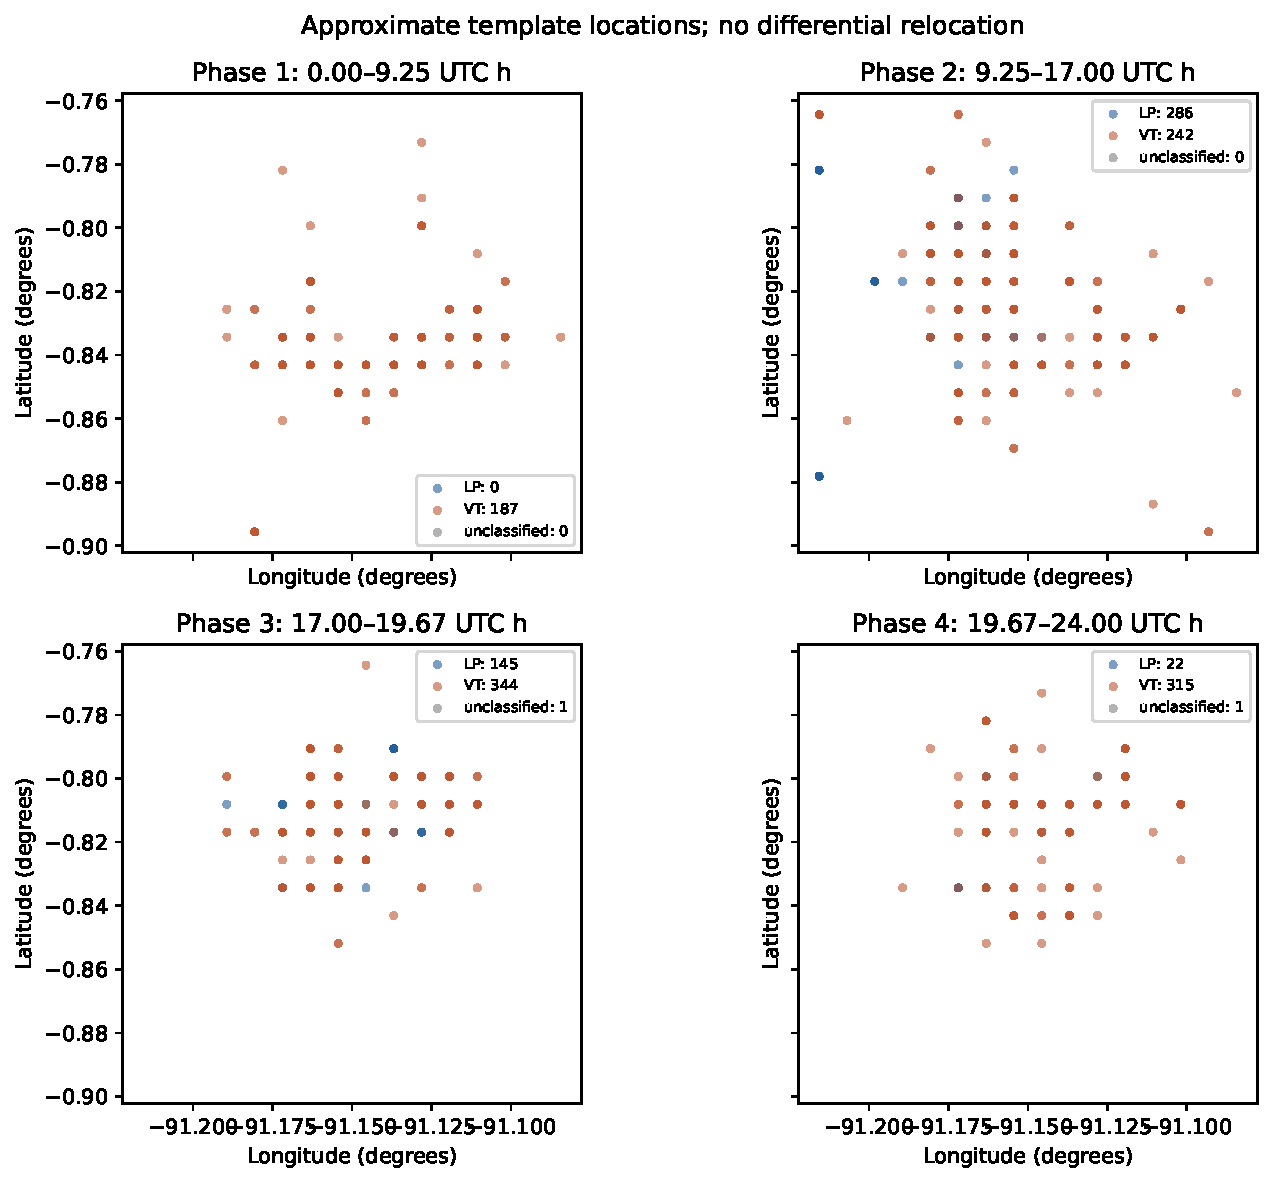
\includegraphics[width=.95\textwidth]{../results/figures/enhanced_phase_maps.pdf}
\caption{Main Figure 4 counterpart with candidate FI classes and inherited approximate locations. Fault traces and differential relocation are missing; a different public surface-elevation model is supplied in the topographic counterpart. Coincident symbols may represent multiple detections co-located with a template.}\end{figure}
\begin{figure}[p]\centering
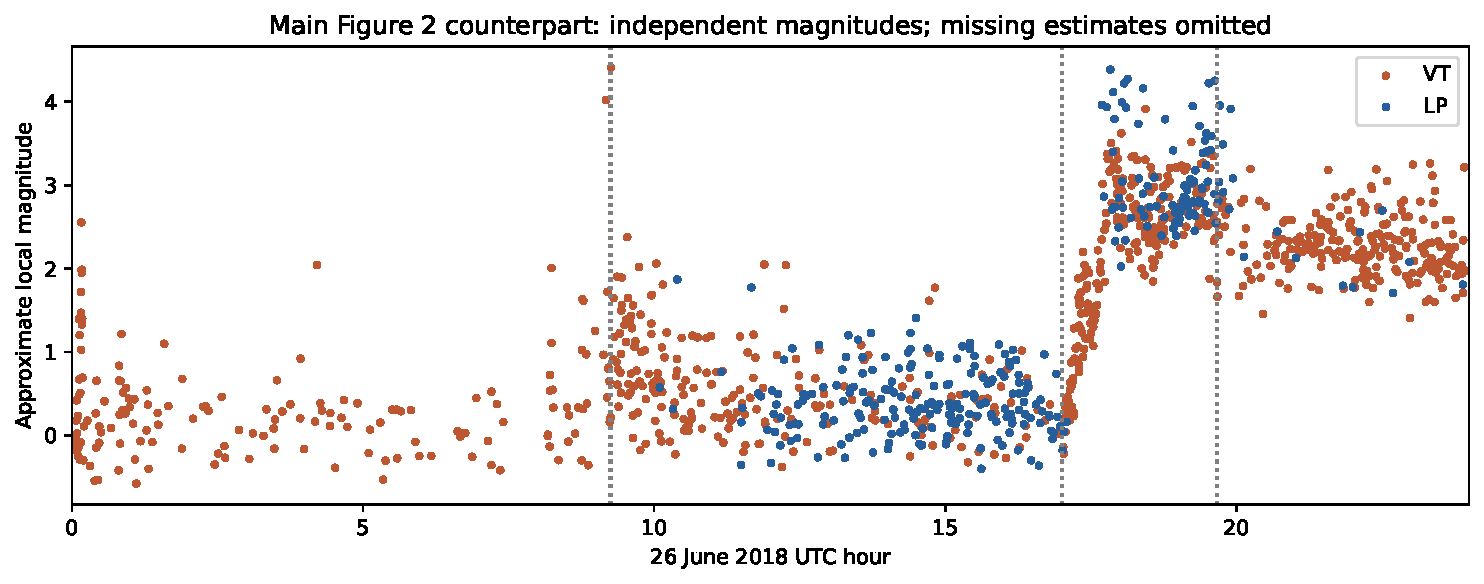
\includegraphics[width=.95\textwidth]{../results/figures/enhanced_magnitude_timeline.pdf}
\caption{Main Figure 2 magnitude--time counterpart. Only the 1154 candidates with approximate magnitude estimates are shown. Absolute response and relative PCA conventions differ from unresolved source controls. GNSS displacement is shown separately in Figure~\ref{fig:gnssppp}.}\end{figure}
\begin{figure}[p]\centering
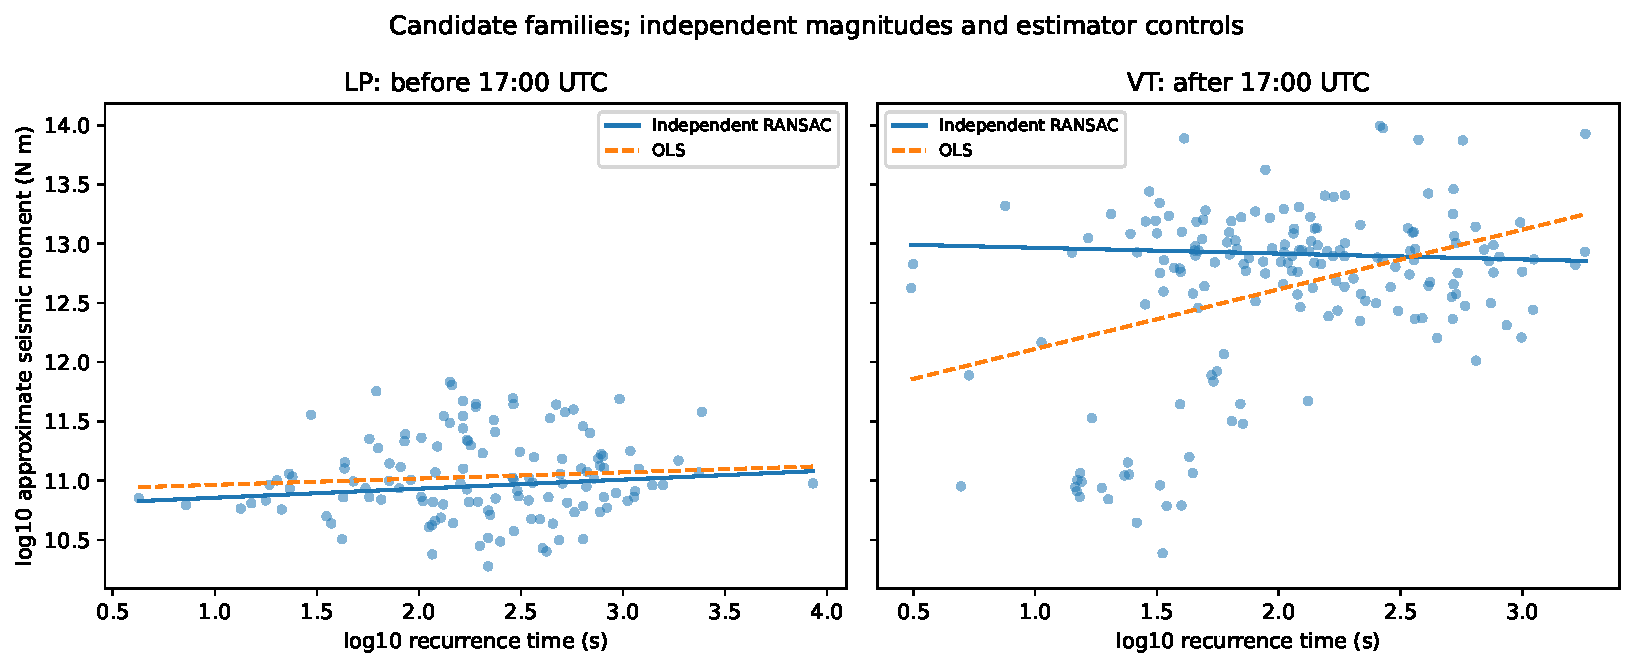
\includegraphics[width=.95\textwidth]{../results/figures/enhanced_permissive_moment_recurrence.pdf}
\caption{Independent main Figure 5 and supplementary S9 counterparts for the permissive one-common-station sensitivity. Approximate moments are paired with preceding recurrence intervals. Independent RANSAC and OLS differ substantially; this is not reproduction of source family memberships or regressions.}\label{fig:moment}\end{figure}
\begin{figure}[p]\centering
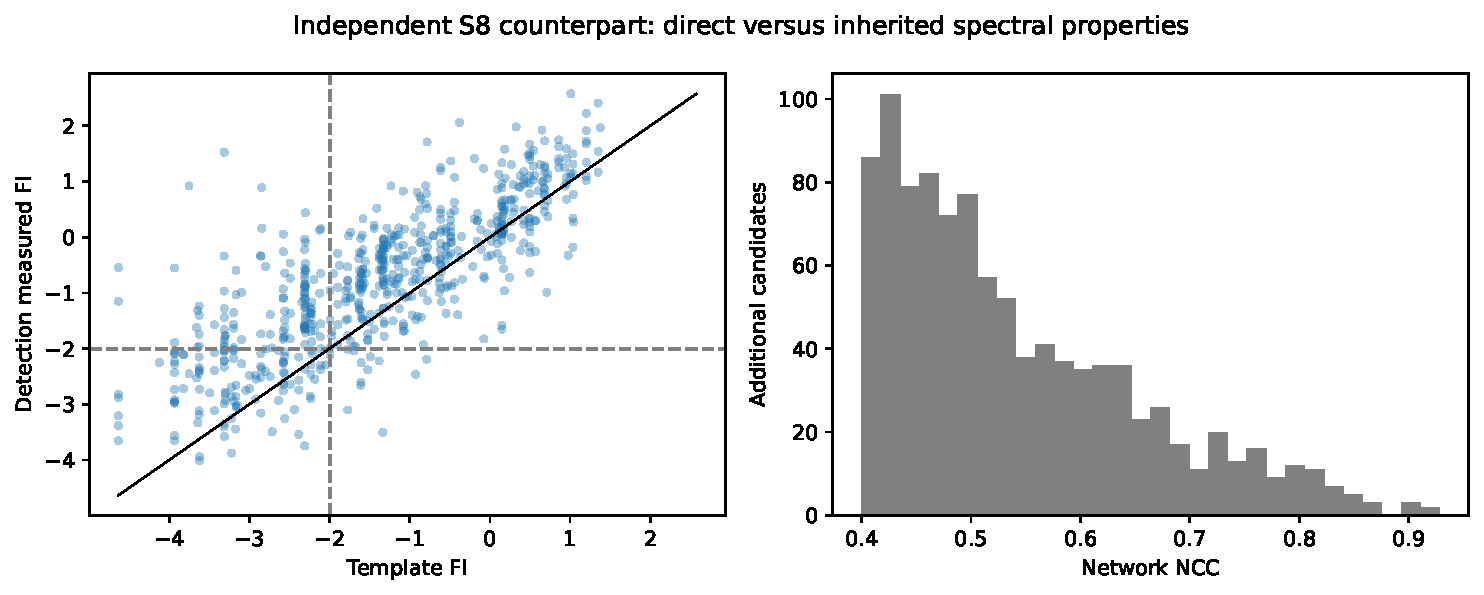
\includegraphics[width=.95\textwidth]{../results/figures/supp_template_fi_comparison.pdf}
\caption{Supplementary S8 counterpart comparing inherited template FI with direct detection FI where measurable. Dashed lines show the LP boundary. Unmeasurable detections are excluded from the scatter, not assigned measured classifications.}\end{figure}

\subsection{Independent geodetic timing sensitivity}
A continuous piecewise-linear bend model is fitted to one-minute median PPP displacement, with a one-minute candidate grid. The primary window spans 14:30--19:15 UTC. GV09 east displacement gives a bend at 17:11 UTC; nine start/end-window choices give 17:09--17:24 UTC. GV03 east displacement bends at 17:38 UTC in the primary window. Other component bends occur from about 15:22 to 18:34 across windows. Therefore, this simple model does not robustly reproduce a unique 17:00 intrusion onset. Postseismic curvature, evolving intrusion and differing station geometry are unresolved; the fitted bend is a statistical description rather than a magma-source inversion.
\begin{figure}[p]\centering
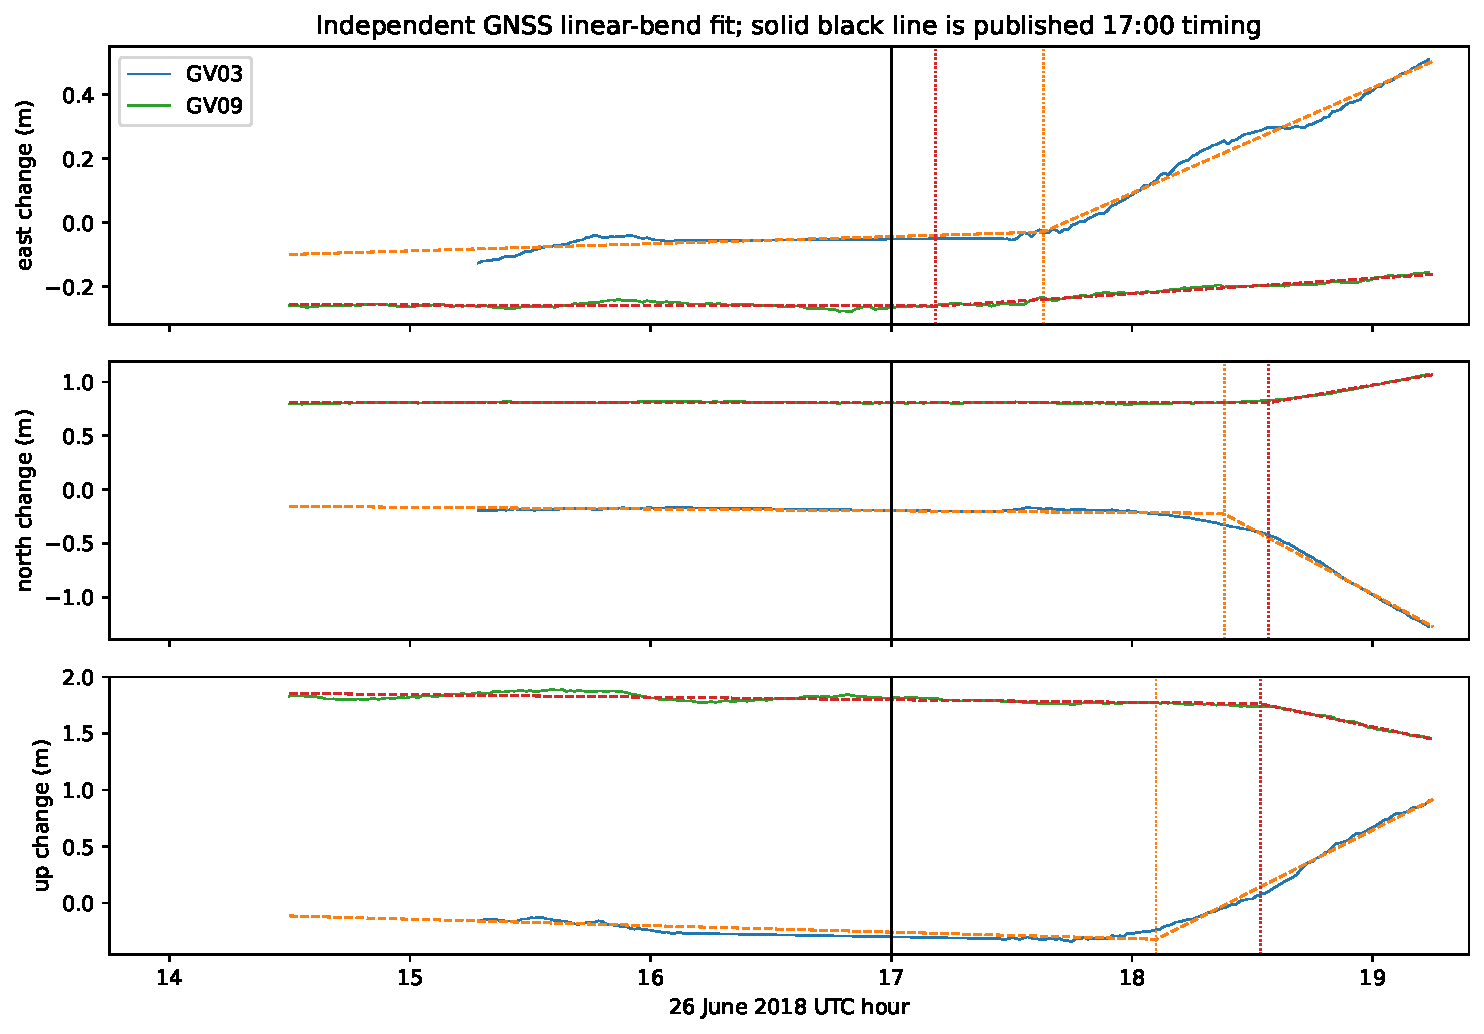
\includegraphics[width=.95\textwidth]{../results/figures/gnss_intrusion_bend.pdf}
\caption{Independent continuous linear-bend fit to screened PPP. Dashed curves are fitted displacements; dotted lines mark component-specific bends. The solid black line marks the published 17:00 intrusion time. The differences and window sensitivity limit timing interpretation.}\end{figure}


\subsection{Numerical surface-elevation counterpart}
A public Copernicus GLO-30 cloud-optimized GeoTIFF \citep{copernicus2026} is retrieved for the Sierra Negra tile and checksummed. The digital surface model includes surface objects and vegetation and has an EGM2008 vertical datum; it is a contextual map, not an eruption-time elevation inversion. It does not change the metadata elevations or approximate location model. Native numerical raster values supply map colour; no published graphic is digitized. Original fault traces and cross-section orientation remain unavailable.
\begin{figure}[p]\centering
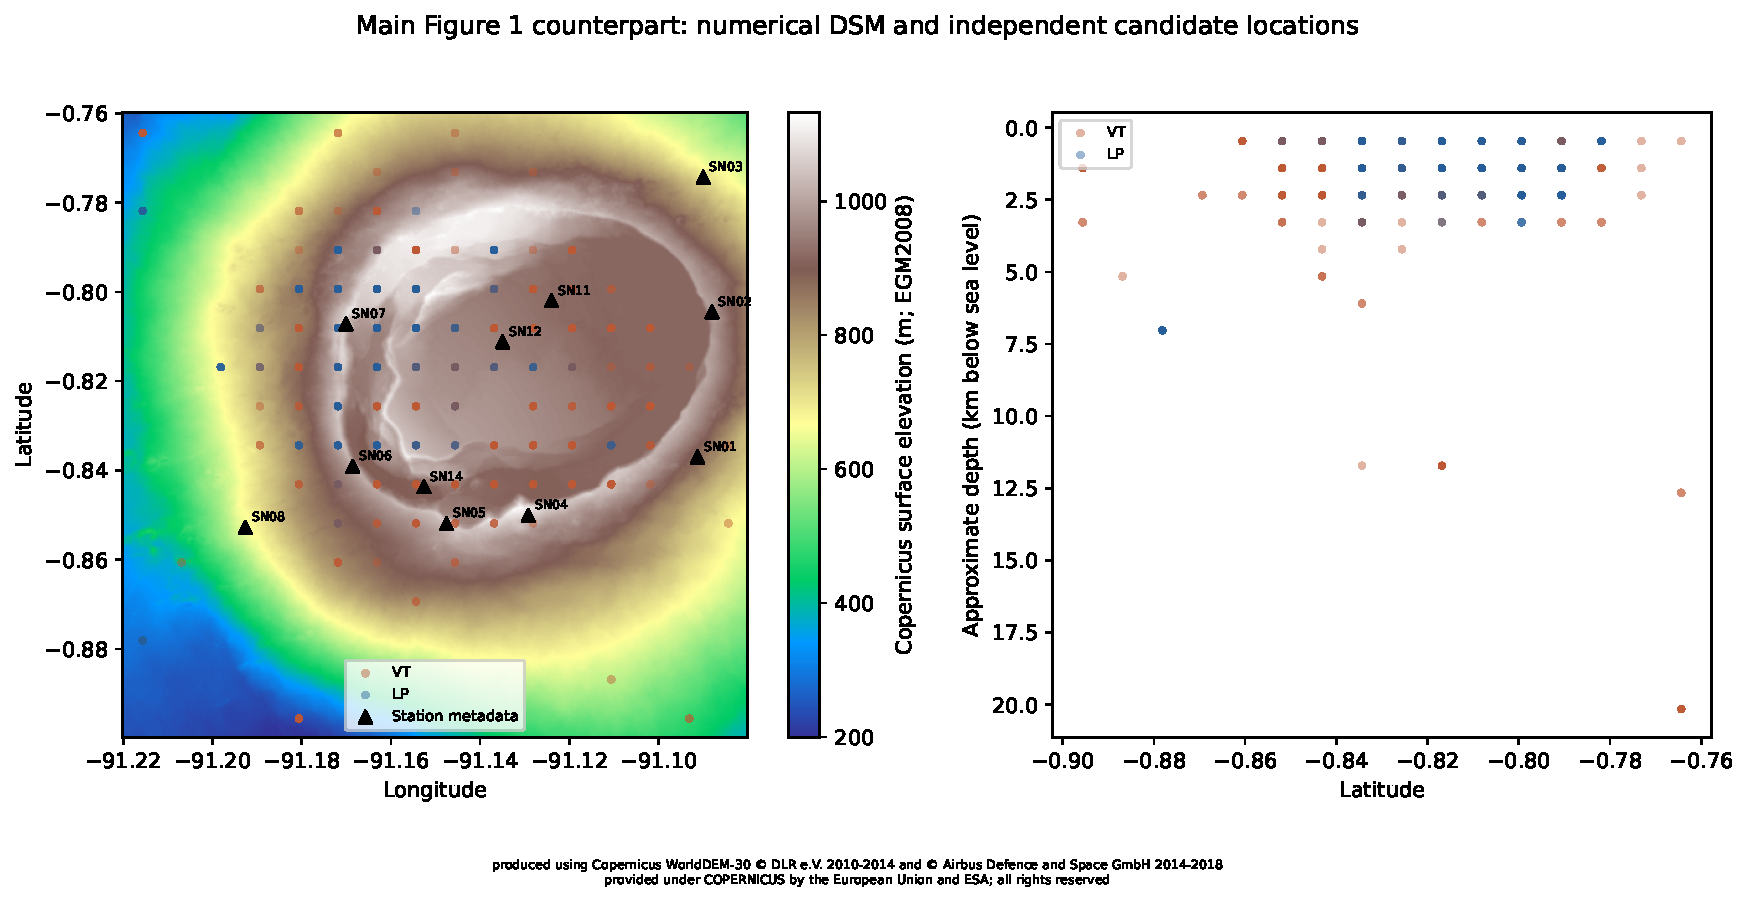
\includegraphics[width=.98\textwidth]{../results/figures/enhanced_topographic_catalog.pdf}
\caption{Main Figure 1 counterpart with public numerical Copernicus surface elevation, station metadata and independent candidate locations. The depth panel is latitude versus approximate depth, not the original fault-perpendicular section. Raw DSM redistribution is excluded from this repository; its retrieval URL, checksum and attribution accompany the figure.}\end{figure}

The permissive family sample contains six LP and eight VT families. Mean recurrence versus population periodicity has Pearson $r=-0.42132$ ($p=0.13352$, $n=14$), differing from the source $r=0.03$. The approximate Fisher 95\% interval is $[-0.77799,0.14071]$. The conditional family percentile bootstrap is asymmetric and should not override the small-sample correlation test. Screen sensitivity and family dependence remain unresolved. The earliest seed LP with at least four qualifying P stations is 10:23:54 UTC but its FI is only $-2.04745$. Requiring the conditional station-bootstrap upper FI bound below $-2$ moves the first seed meeting that rule to 12:07:44 UTC. Therefore, this implementation does not independently establish an onset at exactly two hours after fault slip.


\subsection{Held-out station evidence}
The EC stations SN02 and SN06 do not enter the seven-station template library. Predicted P and S arrivals use the same approximate travel-time model and elevation correction. Availability is restricted to real common three-component intervals, excluding five-second picker blind edges. At the declared 0.5-s tolerance, 440 of 1543 candidates have both P and S support at the same station: 329 seeds and 111 template additions. Waveforms are independent of template construction, although the picker and velocity approximation are shared.

Five hundred within-hour circular time controls preserve catalog clustering through a shared shift in each hour, with independent uniform offsets of 60--3540 s among hours. Real station gaps are reapplied. The mean control support is 14.988 for all candidates and 10.076 for additions; the addition control's central 95\% range is 4.475--16. The empirical upper-tail probability is $1/501$. This comparison supports earthquake-like arrivals for a subset of additions under an approximate within-hour stationarity assumption. It does not calibrate a false-positive rate, establish location accuracy or confirm family membership. Missing support is inconclusive because location errors, gaps and picker sensitivity alter arrival agreement.

\begin{figure}[p]\centering
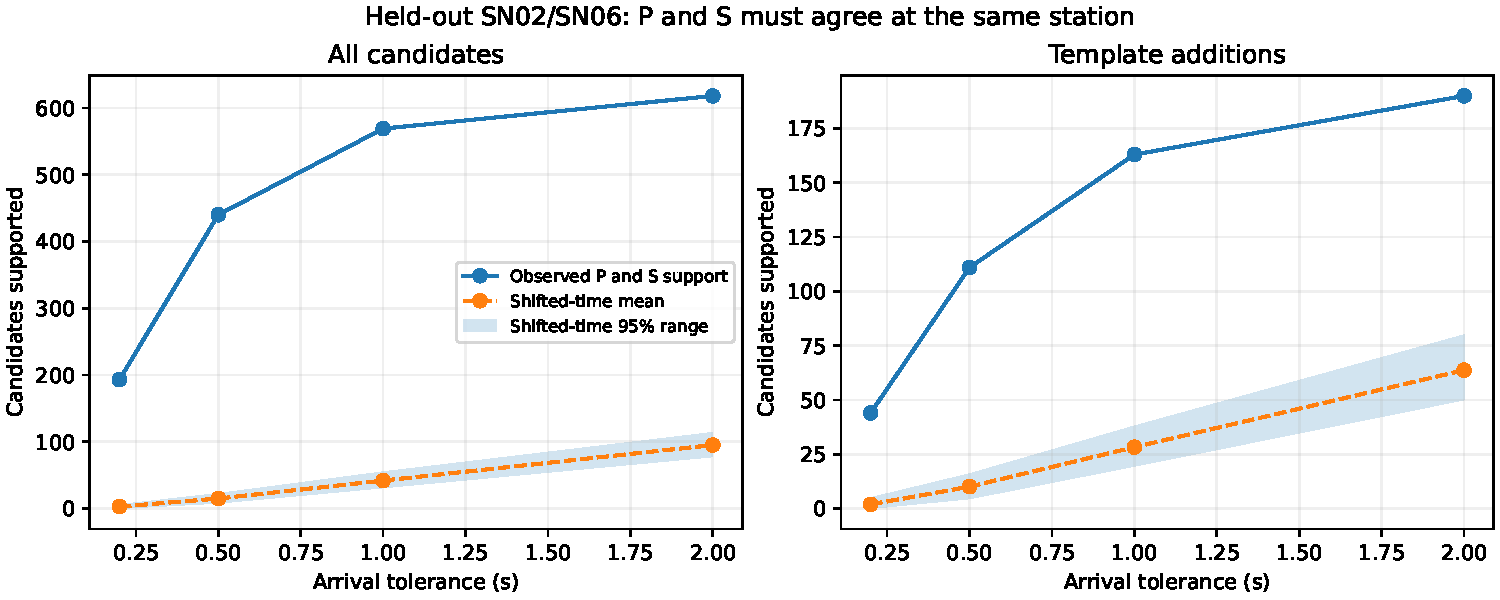
\includegraphics[width=\textwidth]{../results/figures/heldout_station_validation.pdf}
\caption{Independent station evidence for all candidates and template additions. A match requires physically ordered P and S picks at the same held-out EC station. Solid curves show observed support; dashed curves and shading show the mean and central 95\% range of 500 within-hour shifted-time controls. Tolerances are 0.2, 0.5, 1 and 2 s. This is station corroboration rather than a calibrated earthquake false-positive assessment.}\end{figure}


\subsection{Executed differential-location pilot and rejection}
Unmodified HypoDD author code \citep{waldhauser2001} at revision \href{https://github.com/fwaldhauser/HypoDD/tree/fb40407fb768cbdc23a11e27bc841f5d4a98abb7}{\texttt{fb40407fb768}} is compiled with gfortran legacy syntax and the medium memory model. Its unchanged sixteen-event example agrees with the distributed reference to 0.806 m horizontally and 1 m in depth. This check validates the build against an author example; it does not validate the Sierra Negra inputs.

An independent catalog-time-only pilot uses 716 nine-station candidate locations, 151447 event pairs and 1195493 P/S differential observations. Initial pairs are separated by at most 5 km and share at least four station-phase observations. Equal unit P/S weights, ten LSQR iterations and damping 20 are declared alternatives. Tepp Model F nodes become piecewise constant layers, differing from the association's interpolation. Unknown magnitude and input error fields are missing-value placeholders. Cross-correlation differential times, HypoInverse initialization, source bootstrap uncertainty and original controls are absent.

The pilot completes numerically but fails location validation. It retains 206 candidates, of which only three lie within the original search domain. Median horizontal displacement is 35.02 km and median absolute depth displacement is 56.74 km. The graph initially connects 709 events; seven have no accepted pair links. The remaining 503 losses accompany negative-depth flags. The author code's airquake condition checks depth below zero rather than depth below the local volcanic surface. Thus its boundary can reject plausible above-sea-level sources. These outputs are archived as a rejected diagnostic and do not replace the approximate association or template catalog. Numerical completion and smaller differential residuals would not establish physical location accuracy.

\begin{figure}[p]\centering
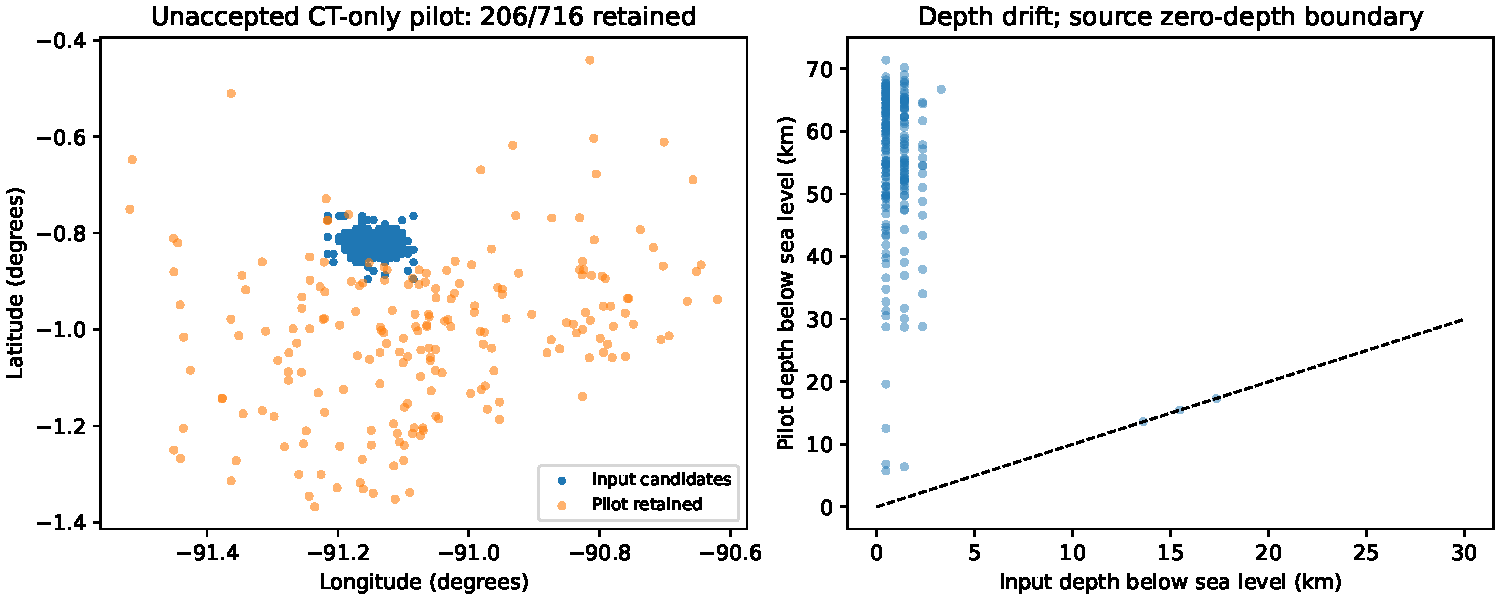
\includegraphics[width=\textwidth]{../results/figures/hypodd_ct_audit.pdf}
\caption{Rejected catalog-time-only HypoDD pilot. Input locations and retained pilot locations are compared geographically (left), and input and final depths are compared with the identity line (right). Large location drift and zero-depth selection prevent accepting this run as a Sierra Negra relocated catalog. Alternative layering and controls differ from the source workflow.}\end{figure}


A boundary sensitivity uses the native IAQ=0 policy. Inspection of the code establishes that this policy freezes negative depth increments rather than allowing above-sea-level sources. All 709 connected events remain, with 700 inside the initial domain. Median horizontal shift is 0.624 km (90th percentile 1.367 km), and median absolute depth shift is 0.355 km. Nevertheless, the largest horizontal shift is 110.62 km and maximum depth is 58.684 km. There are 1219 negative-depth warnings across iterations, which are repeated step flags rather than distinct events. The contrast with the removal run shows strong dependence on the zero-depth boundary. It does not provide independently validated locations or source bootstrap uncertainty; both pilot products remain separate diagnostic catalogs.

\begin{figure}[p]\centering
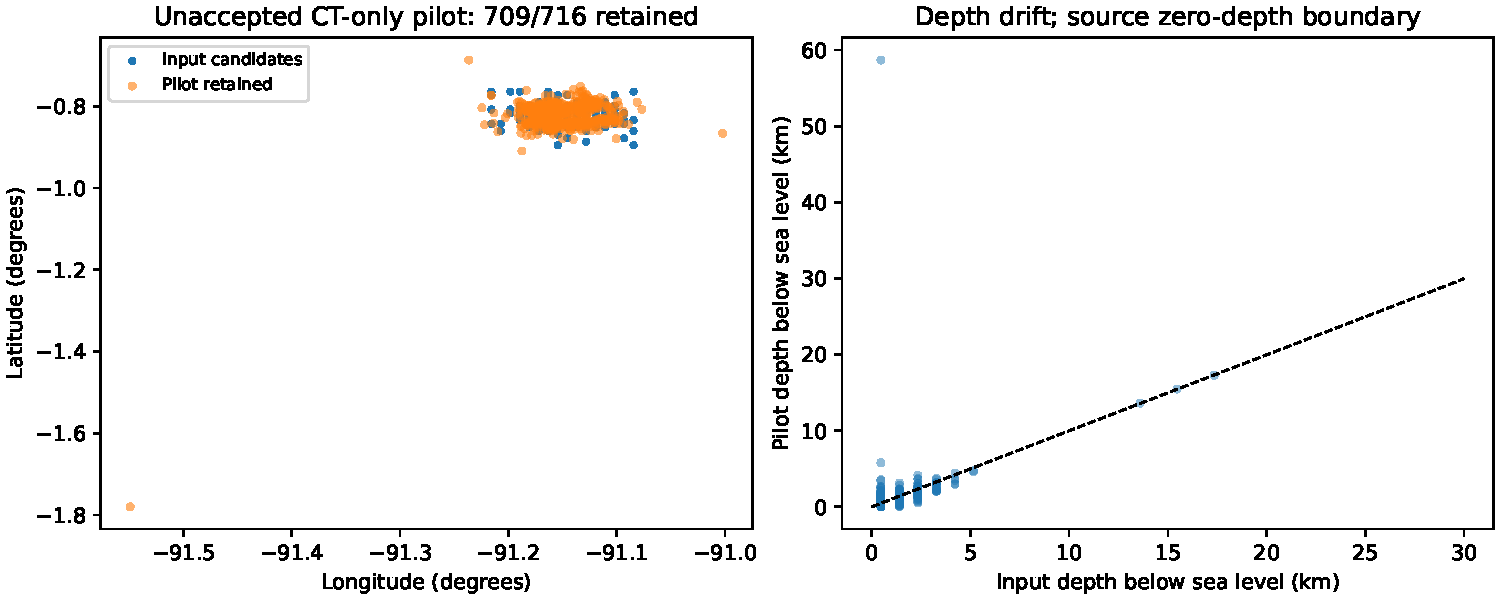
\includegraphics[width=\textwidth]{../results/figures/hypodd_ct_keep_audit.pdf}
\caption{Native zero-depth policy sensitivity for the catalog-time-only pilot. IAQ=0 retains connected events while freezing depth steps that would become negative. Seven hundred of 709 retained events remain within the original domain, but large outliers remain and the zero-depth boundary still restricts the solution. The full geographic extent preserves these outliers. This is a diagnostic catalog rather than a validated reproduction of the original relocated population.}\end{figure}


A fixed-pick audit evaluates absolute arrivals under the association FMM model before and after IAQ=0 relocation. The paired sample comprises 7481 observations across 708 events; 50 observations lack paired predictions within the interpolation domain and are recorded separately. Initial predictions reproduce stored association residuals to 5.73 microseconds. RMS increases from 0.17028 to 0.24721 s, and the fraction within 0.5 s falls from 100\% to 95.95\%. S-phase RMS increases from 0.17505 to 0.28445 s. These are fitted observations rather than independent validation data. Because HypoDD uses a different layer representation, the deterioration does not isolate location error from forward-model mismatch. The output remains an unaccepted diagnostic.

\begin{figure}[p]\centering
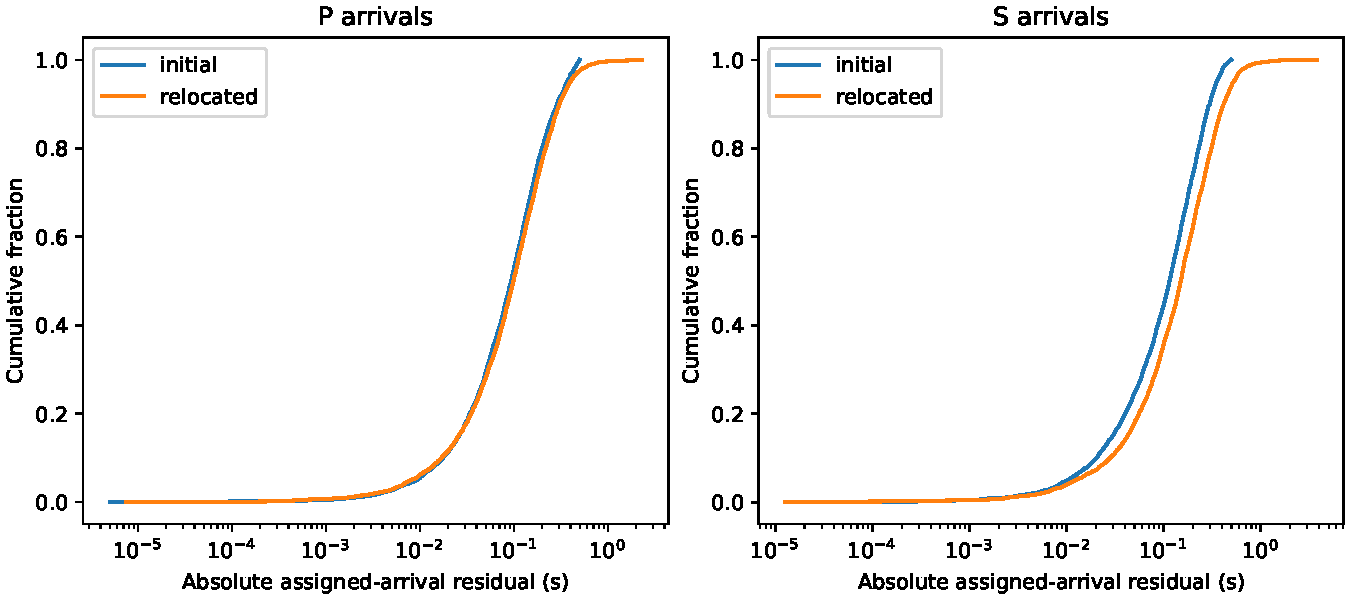
\includegraphics[width=\textwidth]{../results/figures/relocation_absolute_arrivals.pdf}
\caption{Absolute assigned-arrival residual distributions for P and S phases. Initial and native IAQ=0 pilot locations predict the same original picks with the association FMM model and identical elevation corrections. Horizontal axes show absolute residual in seconds on a logarithmic scale; vertical axes show cumulative fraction. Only observations with both predictions within the interpolation domain enter the paired comparison. The changed residual distributions assess consistency with the initial model, not independent location accuracy.}\end{figure}

\section{Comparison with published results}
The comparison table in the repository distinguishes uncomputed quantities from numerical disagreements. The accessible paper reports two inconsistent VT counts: 1,224 in Results and 1,214 in Methods. With 711 LP events, the first total is 1,935 and the second is 1,925. Independently, 694 located events plus 1,241 new template detections sum to 1,935. We preserve both reported counts and request source catalog reconciliation before selecting a target.

\begin{table}[ht]\centering\small
\begin{tabular}{p{.38\textwidth}p{.20\textwidth}p{.30\textwidth}}\toprule
Quantity & Published & Present calculation\\\midrule
Enhanced event total & 1,935 by stated workflow & 1,543 independent candidates\\
VT classifications & 1,224 / 1,214 & 1,088 inherited labels\\
LP classifications & 711 & 453 inherited labels\\
Families / member events & 29 / 714 & 2 / 23; sensitivity 14 / 452\\
Anti-correlated LP pairs & 11 & 5 review candidates\\
VT / LP regression $R^2$ & 0.70 / 0.07 & OLS sensitivity 0.148 / 0.007\\
Fault earthquake time & 09:15 UTC & Original entry 09:15:32.299\\
GV09 vertical hourly change & At least 1.83 m & 1.86707 m, independent PPP\\
Original catalog subset & Archive rows for date & 219 events recovered\\\bottomrule
\end{tabular}
\caption{Comparison targets from \citet{song2026} and computations from the original archive. The 219 original events are not a numerical estimate of enhanced-catalog completeness. No difference is assigned to uncomputed quantities.}
\end{table}

Exact agreement of the enhanced waveform results is not testable here. Independent counterparts of main Figures 3 and 5 use measured spectra, computed candidate families and approximate magnitudes; original memberships and waveform identities remain unavailable. The reviewed supplement contains S1--S9. We reproduce all four PAYG ground-velocity day plots in S5 from archived waveforms and epoch responses (Figure~\ref{fig:payg}); Independent distribution, negative-pair and direct-versus-inherited FI counterparts are also calculated; source calibration examples and precise memberships remain unavailable. S9 fits log--log moment and recurrence time using RANSAC. Its unspecified estimator controls prevent exact regression agreement; both OLS and independently specified RANSAC are evaluated where candidate family data support a fit.

\section{Discussion}
Figure~\ref{fig:concept} is an original schematic separating recorded seismic observations from the proposed physical sequence. A delayed response could be consistent with local changes in fault conditions, but the original catalog alone does not measure fluid pressure, flux, or effective stress. The waveform and geodetic counterparts constrain timing, but unresolved source membership, location and processing differences prevent an exact test of the proposed mechanism.

\begin{figure}[p]\centering
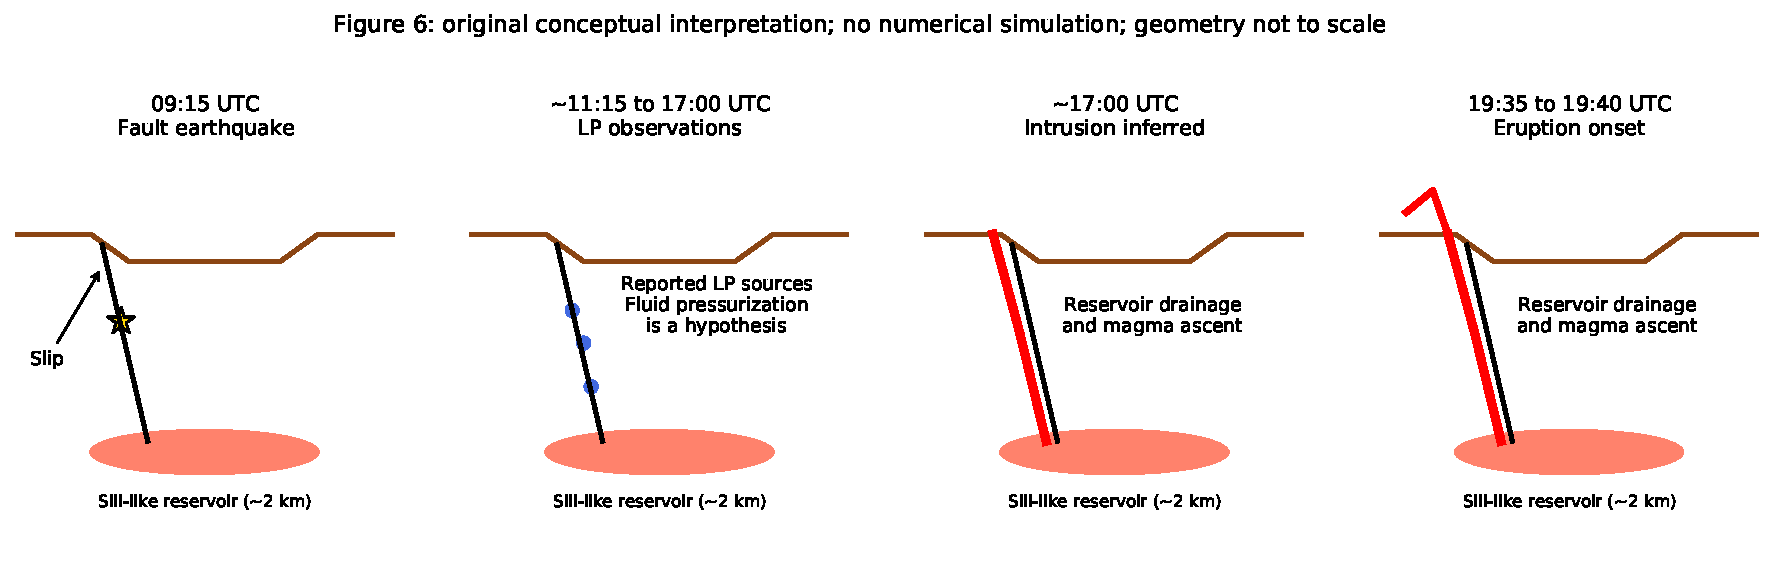
\includegraphics[width=\textwidth]{../results/figures/fig06_conceptual_sequence.pdf}
\caption{Original conceptual interpretation corresponding to main Figure 6. The panels depict fault slip, a proposed intervening fluid process associated with reported LP sources, intrusion, and eruption. Times are taken from the literature, including its 19:35--19:40 onset range. Geometry is not to scale. Fluid pressurization is a hypothesis; this is neither a numerical simulation nor an independently measured pressure history.}
\label{fig:concept}\end{figure}

A rigorous recurrence analysis must also consider missed events, temporal censoring, magnitude uncertainty, and dependence among events in the same family. These effects can alter a moment--recurrence regression even when pointwise numerical methods are correct. Leave-one-out resampling of individual events does not account for all family-level dependence. Future observational execution should compare both interval-pairing conventions, quantify family-level uncertainty, and inspect how frequency bands and station weights alter classifications and membership.

\section{Limitations}
Network access permits archive downloads, although some endpoints still fail. The modern Python environment includes ObsPy, PyTorch, SeisBench and PyOcto. The public GitHub repository is created and its pushed commit verified at \href{https://github.com/maochuan-zhang-UW/song2026-sierra-negra-reproduction}{the public project repository}. VCH1 waveforms (skipped at the user's instruction), SN02 gaps and source controls limit an exact enhanced-catalog reproduction. EC data are now picked and associated in the separate nine-station coverage experiment. EarthScope authentication permits verified observation and navigation downloads. ESA precise orbit and clock products and IGS20 antenna calibration support independent float PPP. Historical login redirects remain in the acquisition audit but no longer describe the current access status.

The supplement has been reviewed and archive checksums and license are verified. Source depth datum and location-error units remain unresolved. The enhanced candidate population is independently calculated, but exact source membership, confirmed source polarity reversals and published regression agreement are not claimed. High-rate GNSS solutions are independently computed with different software and corrections. Independent response stabilization and graphical gain choices limit amplitude comparison for the reproduced PAYG figure.

\section{Conclusions}
We recover 219 archived original events, associate 716 approximate nine-station candidates and compute a 1.867-m GV09 hourly vertical change at the fault earthquake. A separate seven-station full-day template search expands 536 seeds to 1543 candidates, with inherited labels of 453 LP, 1088 VT and two unclassified events. Every selected template recovers itself; direct spectra disagree with inherited type in 126 of 646 measurable additional events. The primary graph yields two LP families with 23 members, while a permissive screen yields fourteen families with 452 members. Therefore, candidate counts and membership depend on coverage and processing choices.

Independent approximate magnitudes and recurrence fits show weak LP moment--recurrence association and a positive VT OLS slope under the permissive screen, but the published regression statistics and robust-fit contrast are not reproduced. Geodetic bend timing varies among components and windows. Original relocation, calibration and manual controls remain gaps; correlation and timing do not uniquely establish a fluid-triggering mechanism. The code, executed notebook, numerical data products and partial figure counterparts provide a reusable basis for comparisons when source controls become available.

\appendix
\section{Supplementary counterparts}
The following independent plots use computed observations. S1 calibration-event identities and S6 source amplitude--magnitude calibration samples remain unavailable, so those source panels are not reproduced. The FI histogram supplies a partial distribution counterpart only. Nearest-event distances use an explicitly approximate three-dimensional local Cartesian metric. Inherited positions can create coincident points; these distances are not independent relocated separations. Histogram modes use 0.1-magnitude bins without an empirical offset and describe magnitude-estimated subsets, not independently demonstrated catalog completeness.

\begin{figure}[p]\centering
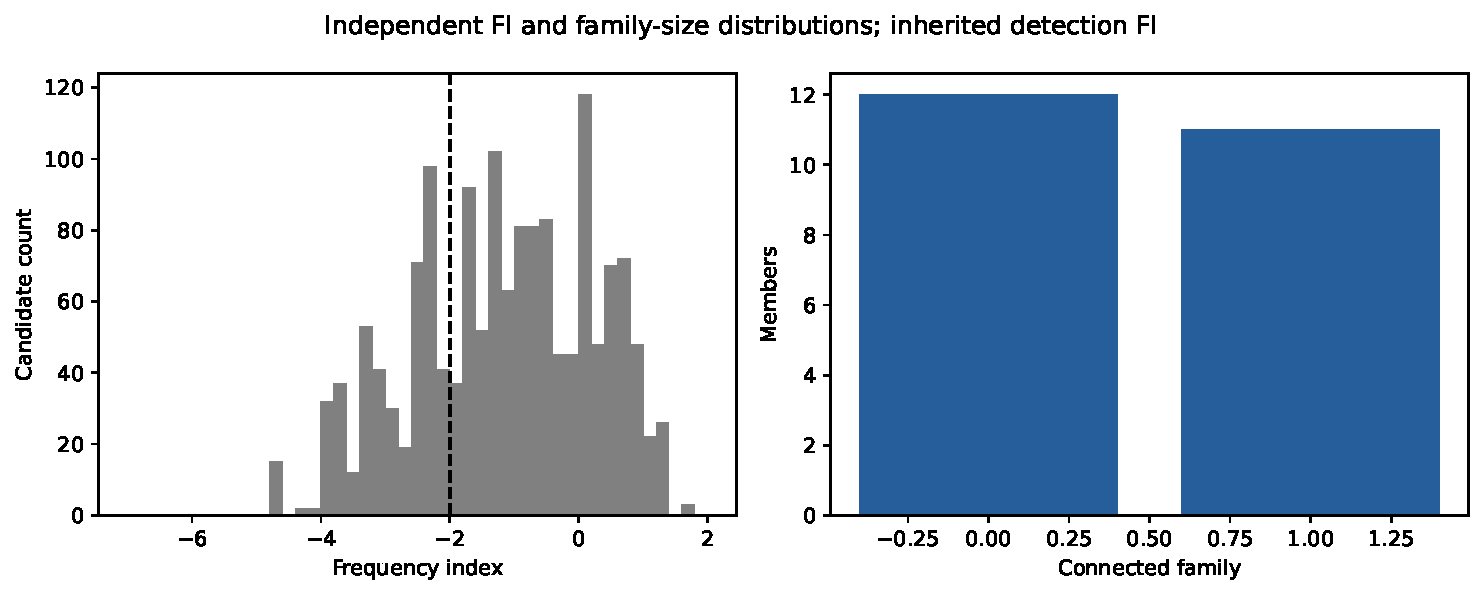
\includegraphics[width=.95\textwidth,height=.80\textheight,keepaspectratio]{../results/figures/supp_candidate_distributions.pdf}
\caption{Partial S1 distribution counterpart and family-size distribution. Original hand-selected calibration waveforms are absent.}\end{figure}

\begin{figure}[p]\centering
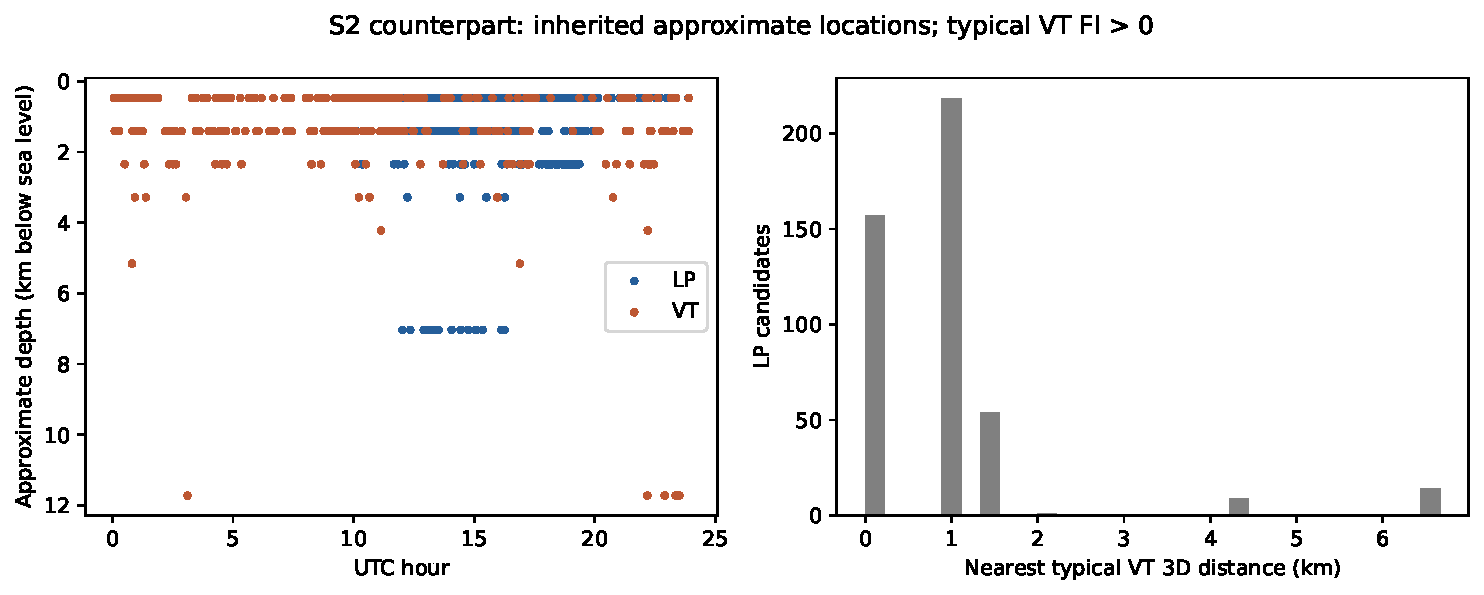
\includegraphics[width=.95\textwidth,height=.80\textheight,keepaspectratio]{../results/figures/supp_spatial_LP_VT.pdf}
\caption{S2 counterpart using FI-greater-than-zero typical VT candidates and approximate inherited locations. The histogram uses nearest three-dimensional distances in kilometres.}\end{figure}

\begin{figure}[p]\centering
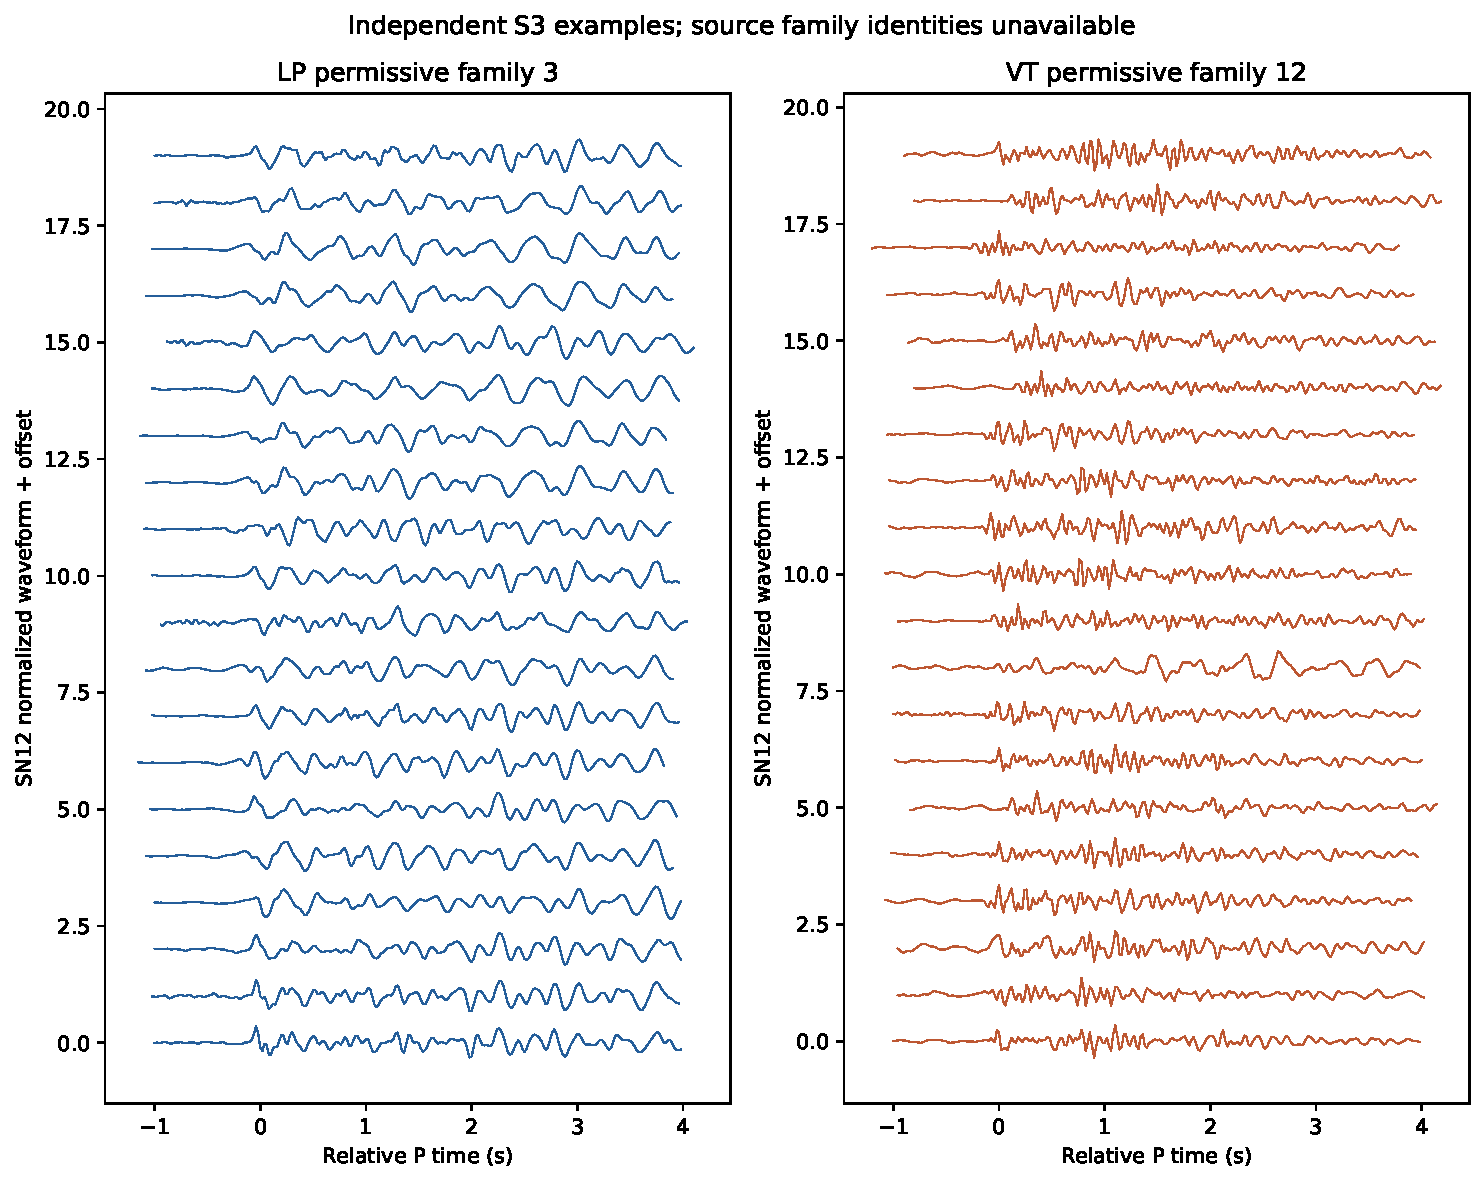
\includegraphics[width=.95\textwidth,height=.80\textheight,keepaspectratio]{../results/figures/supp_family_waveforms.pdf}
\caption{S3 counterpart: independently selected permissive LP and VT family examples at SN12/Z, normalized and aligned with maximum positive correlation within 0.2 s. Original family identities are unavailable.}\end{figure}

\begin{figure}[p]\centering
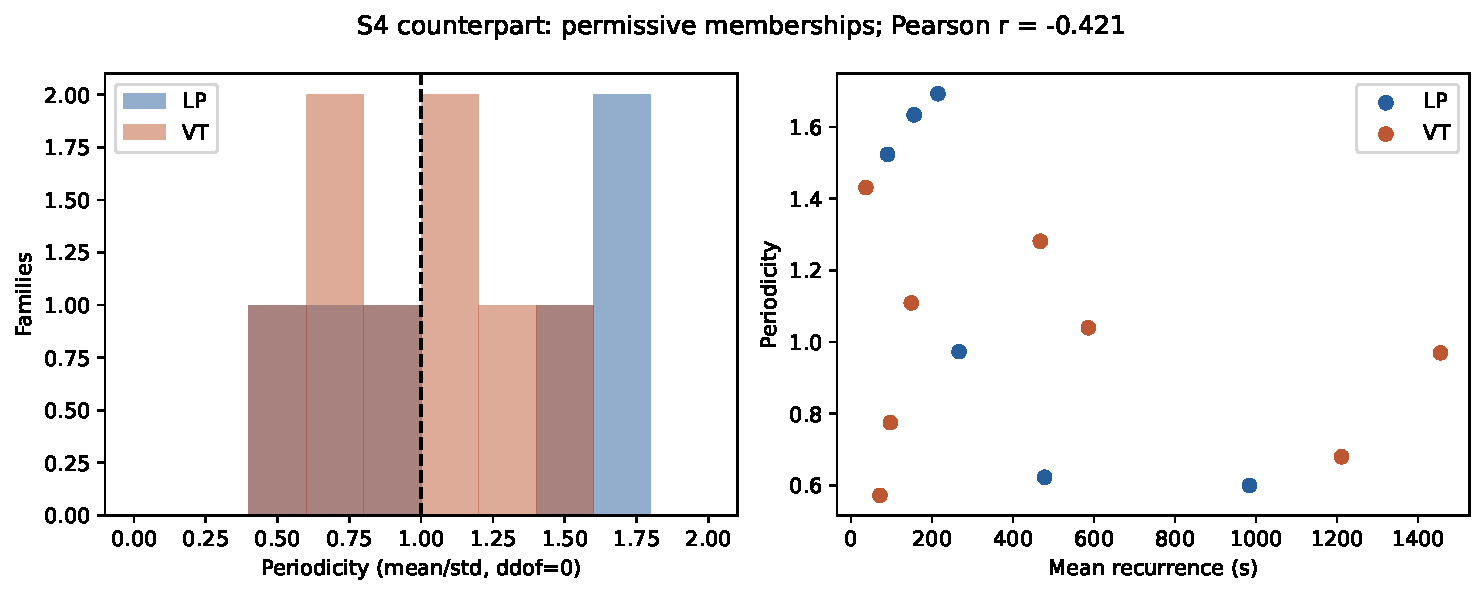
\includegraphics[width=.95\textwidth,height=.80\textheight,keepaspectratio]{../results/figures/supp_family_periodicity.pdf}
\caption{S4 counterpart: population-standard-deviation periodicity and mean recurrence for the permissive fourteen-family sample. Screening uncertainty is larger than plotting precision.}\end{figure}

\begin{figure}[p]\centering
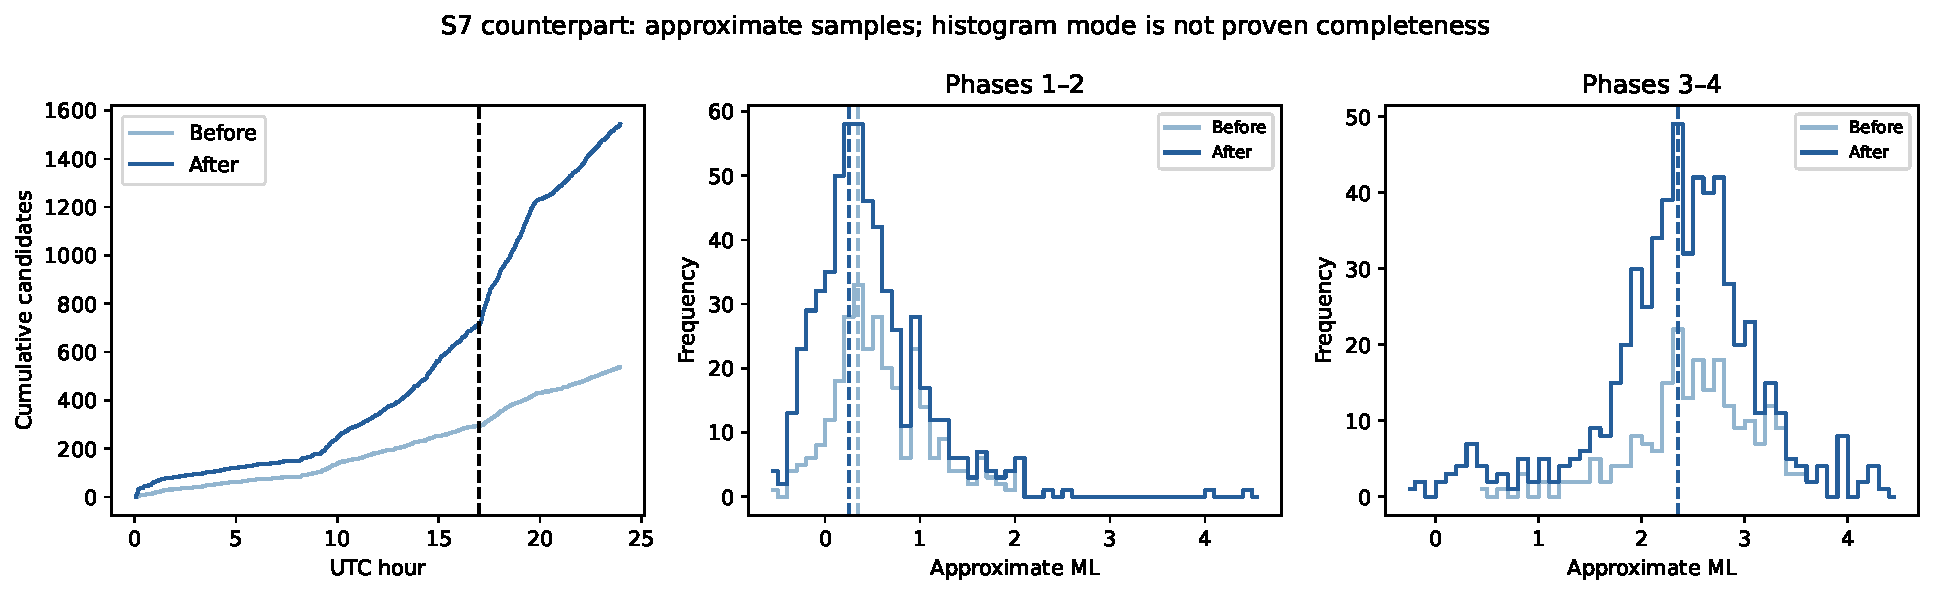
\includegraphics[width=.95\textwidth,height=.80\textheight,keepaspectratio]{../results/figures/supp_before_after_matching.pdf}
\caption{S7 counterpart: candidate counts and magnitude histograms before and after matching. Dashed histogram lines indicate uncorrected modal-bin magnitudes, not proven completeness thresholds.}\end{figure}

\begin{figure}[p]\centering
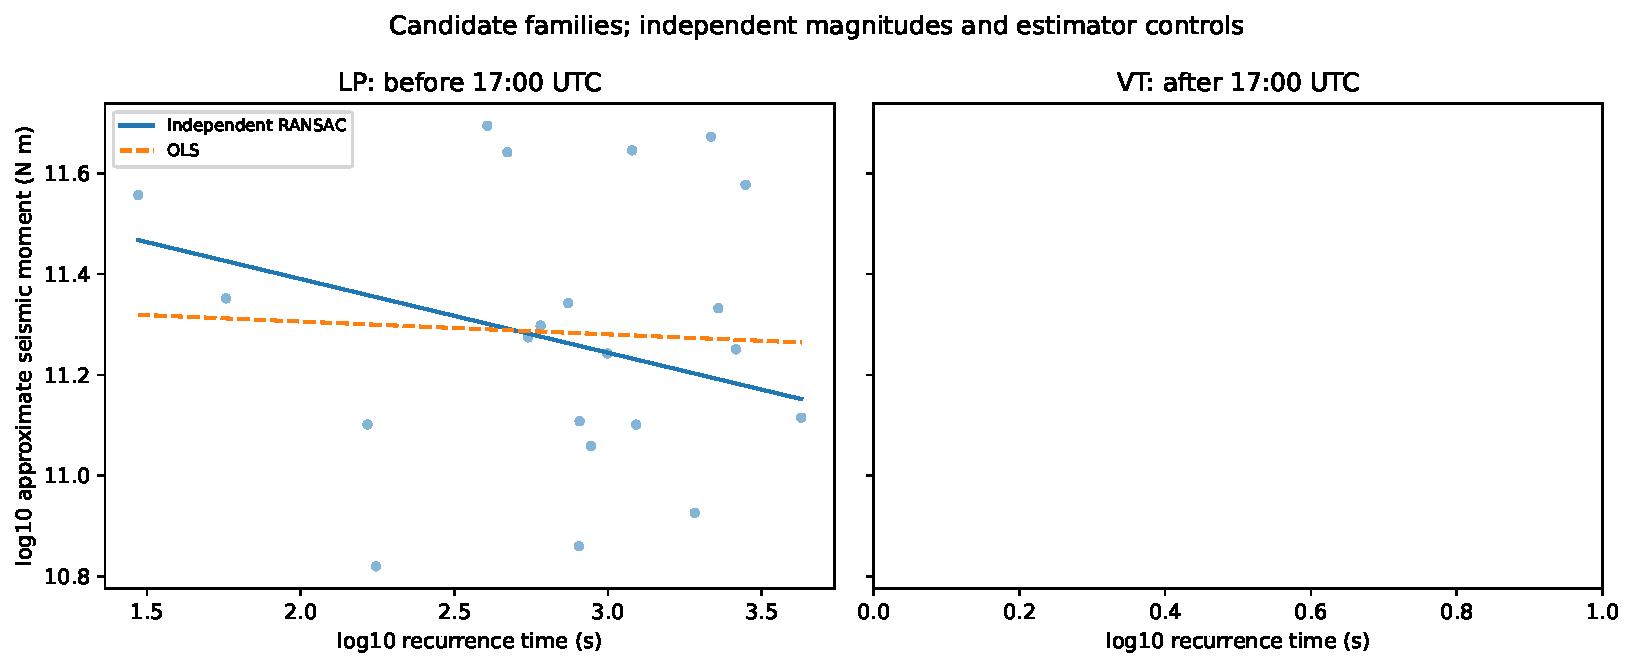
\includegraphics[width=.95\textwidth,height=.80\textheight,keepaspectratio]{../results/figures/enhanced_moment_recurrence.pdf}
\caption{Primary four-common-station moment--recurrence analysis. No qualifying VT family exists under this screen, so the VT panel cannot test the source contrast.}\end{figure}

\begin{figure}[p]\centering
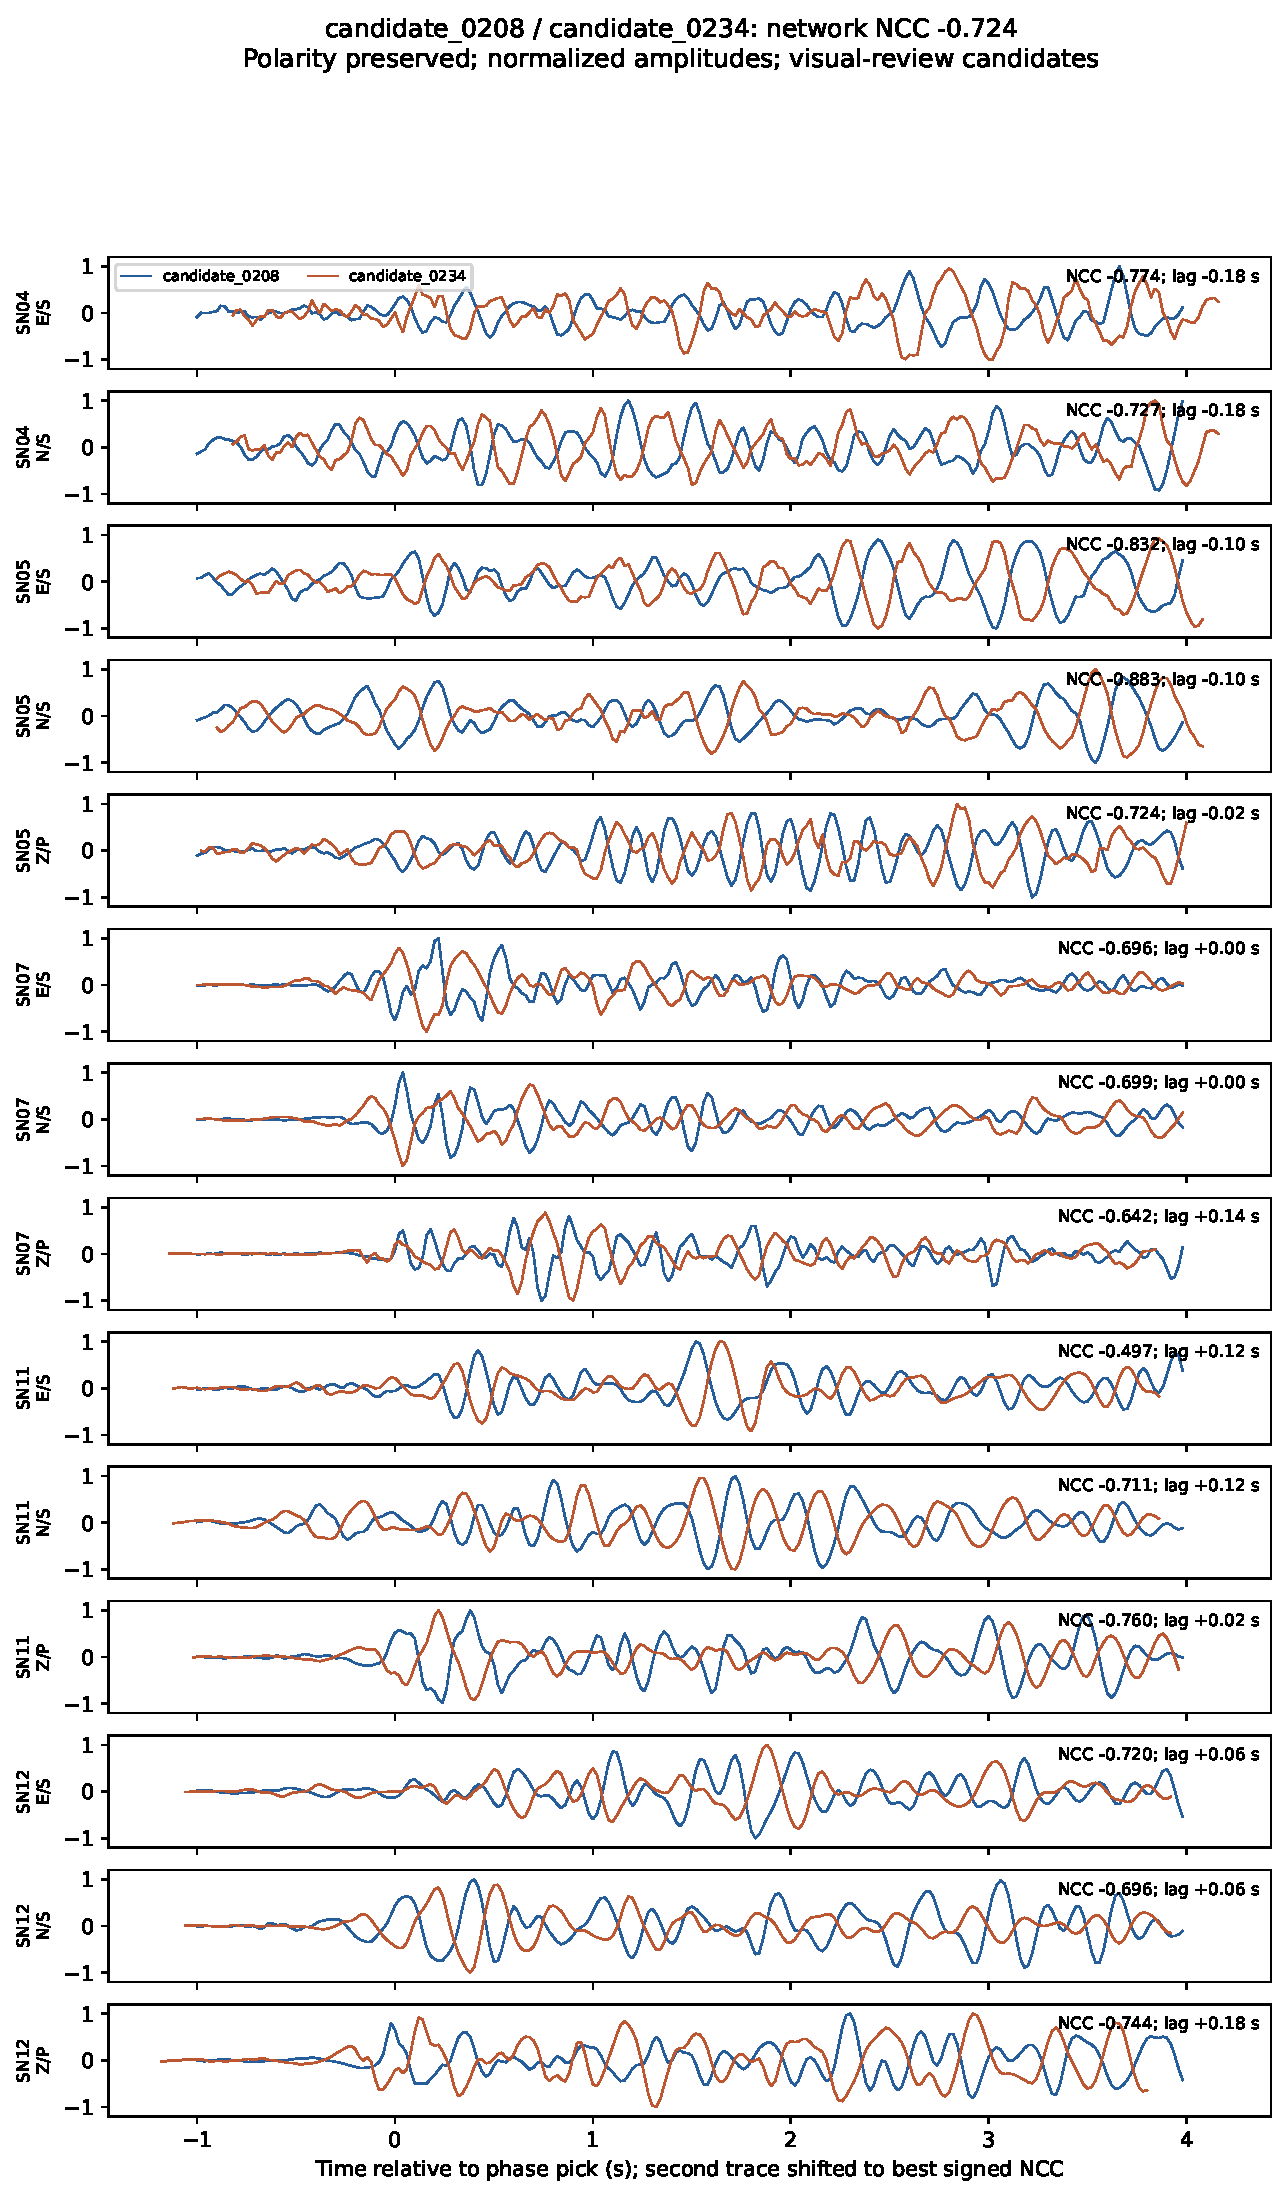
\includegraphics[width=.95\textwidth,height=.80\textheight,keepaspectratio]{../results/figures/negative_pair_0208_0234.pdf}
\caption{Polarity-preserving baseline waveform overlay for candidates 0208 and 0234. Channel-specific signed NCC and lags are indicated. Negative coefficients require source-polarity review.}\end{figure}

\begin{figure}[p]\centering
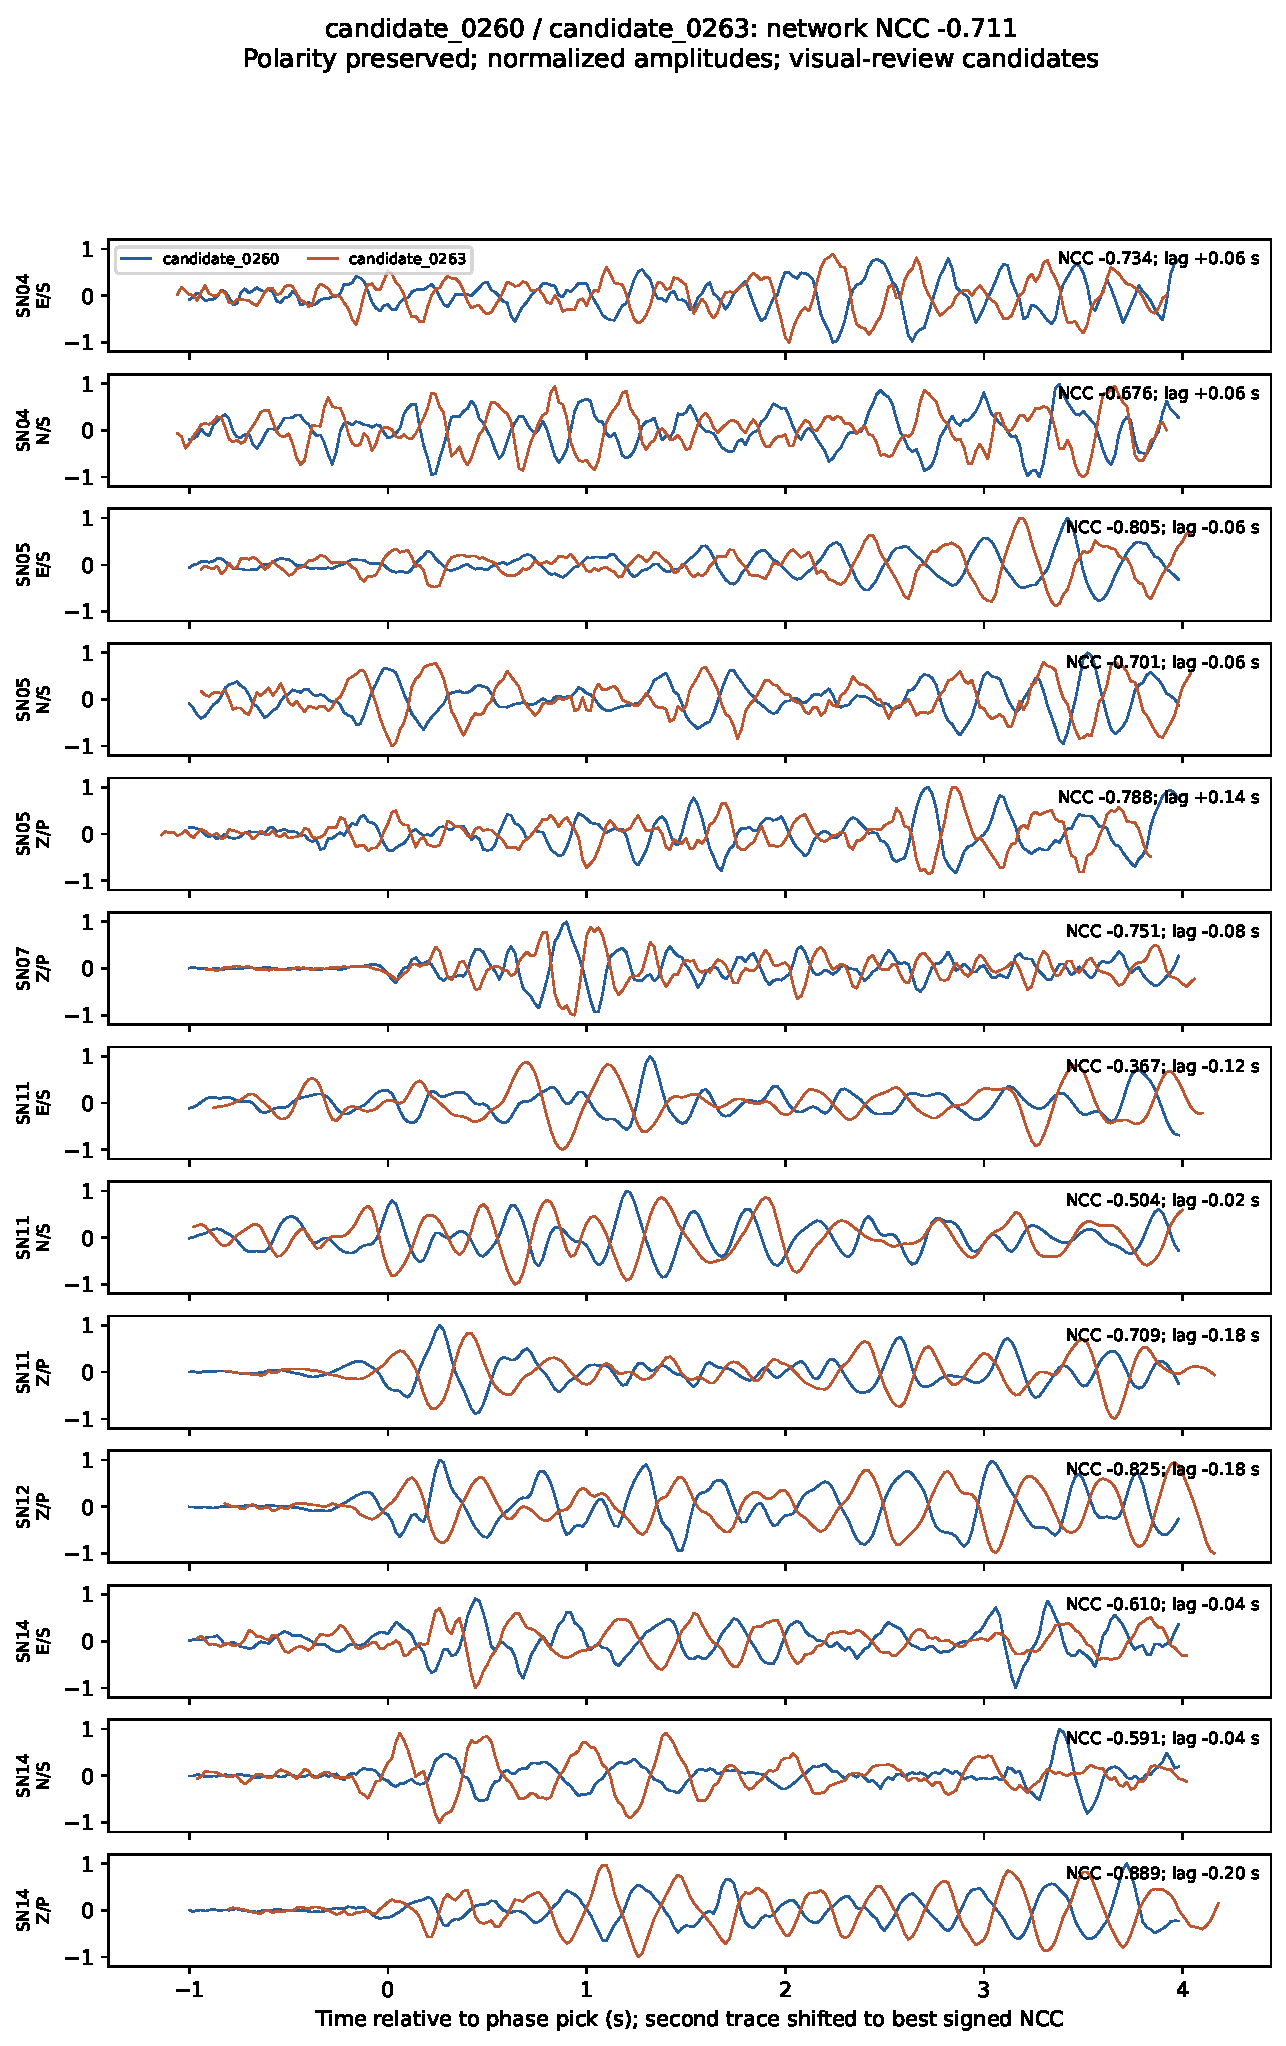
\includegraphics[width=.95\textwidth,height=.80\textheight,keepaspectratio]{../results/figures/negative_pair_0260_0263.pdf}
\caption{Polarity-preserving baseline waveform overlay for candidates 0260 and 0263; an independent review example, not the source event pair.}\end{figure}

\begin{figure}[p]\centering
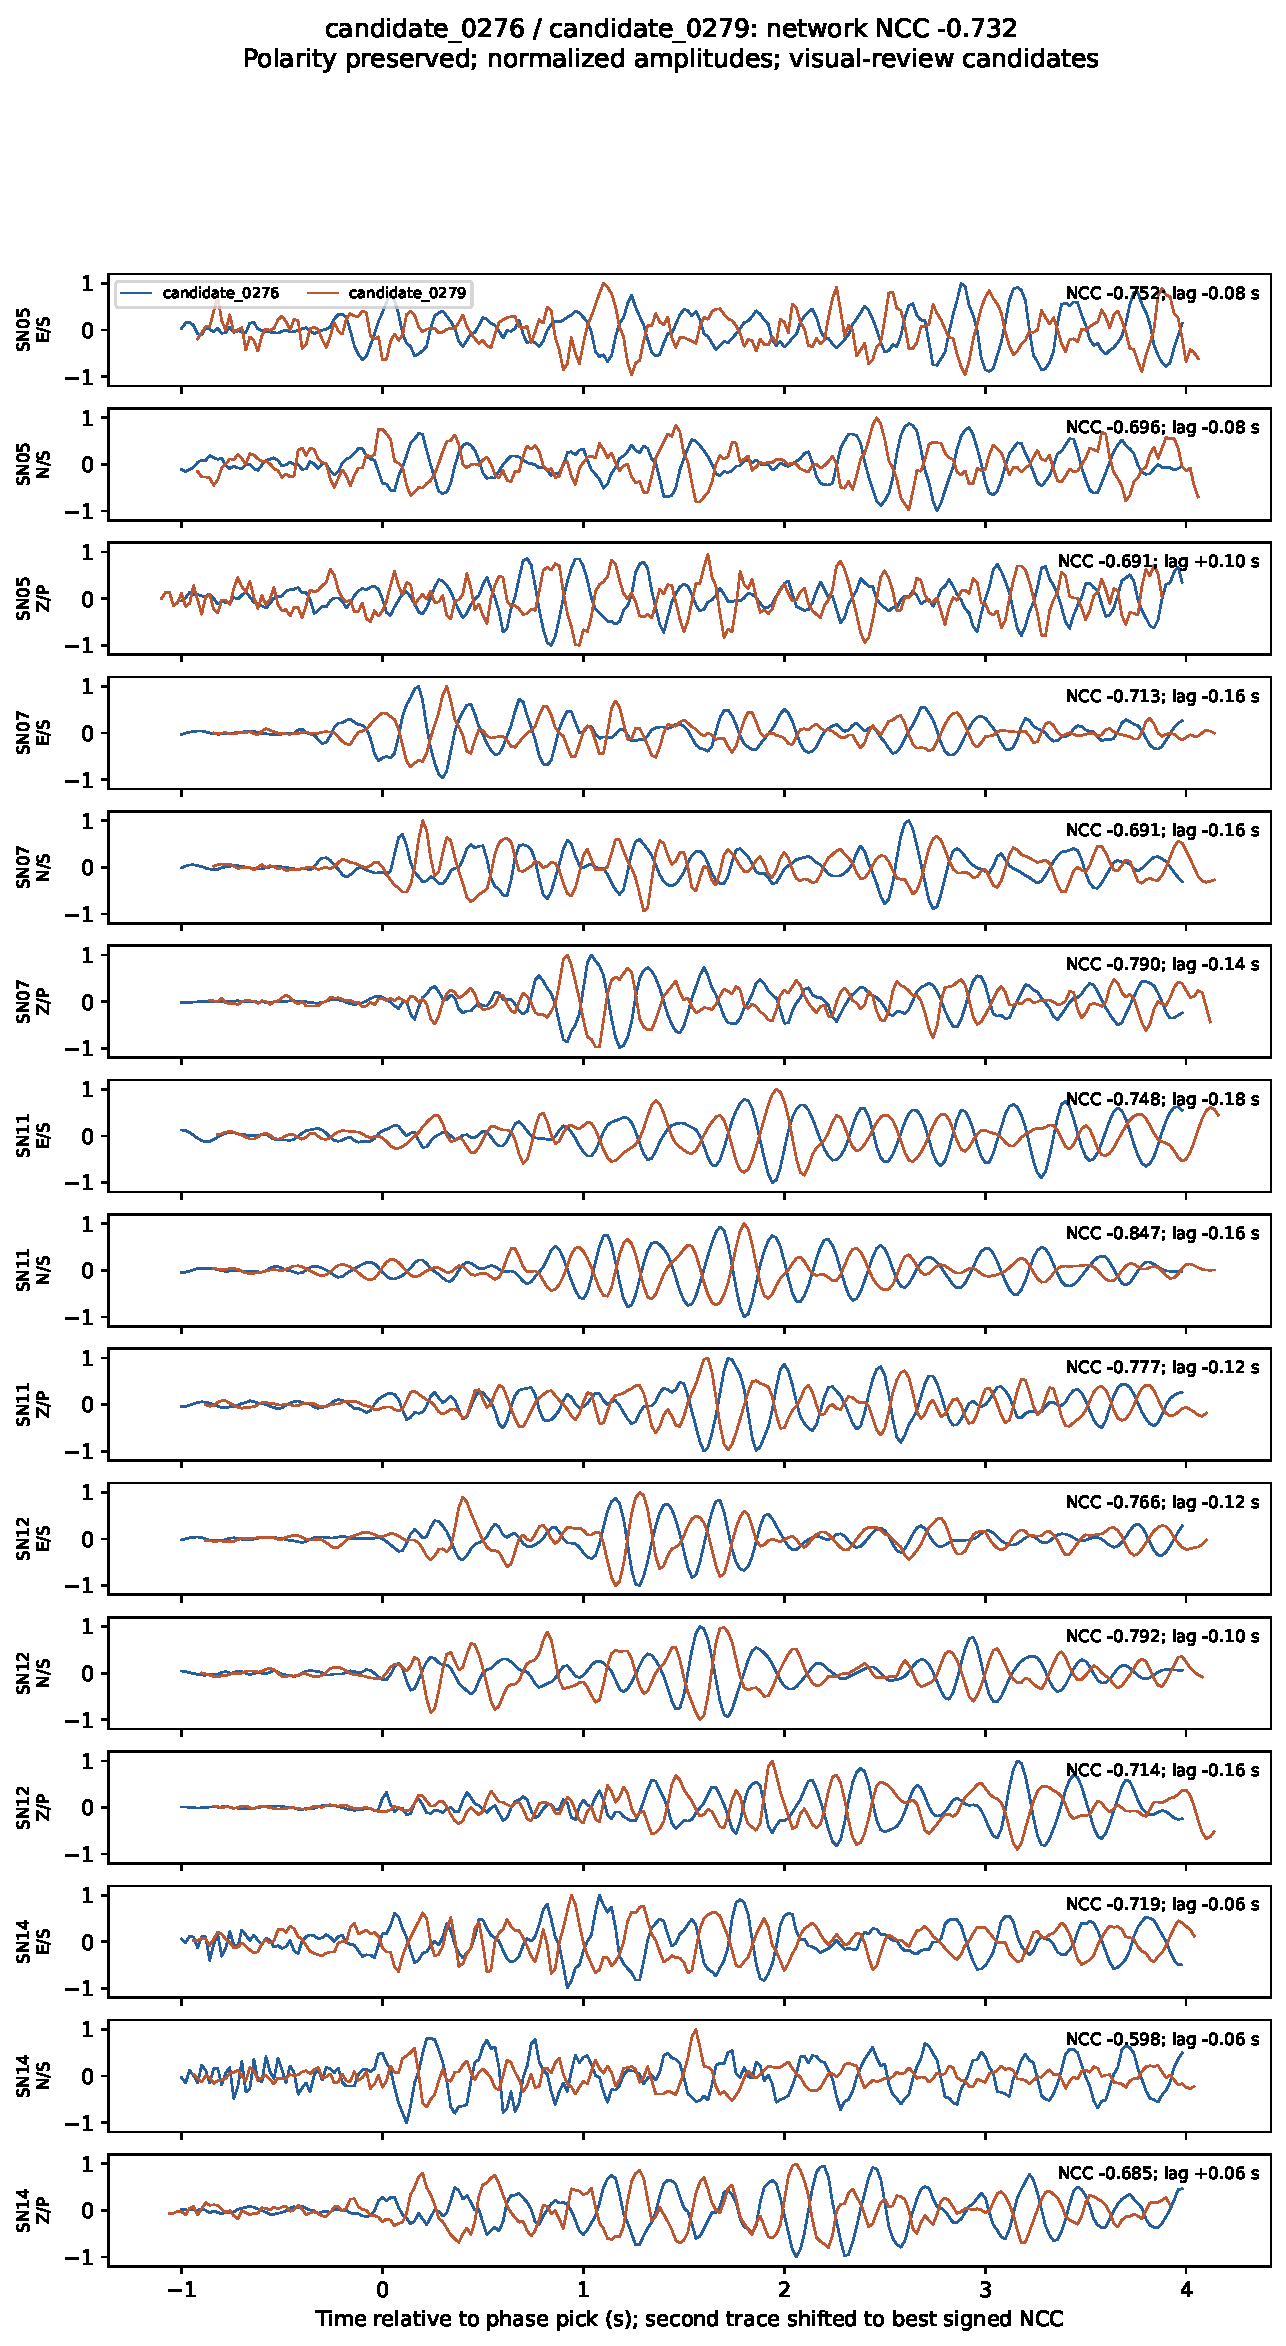
\includegraphics[width=.95\textwidth,height=.80\textheight,keepaspectratio]{../results/figures/negative_pair_0276_0279.pdf}
\caption{Polarity-preserving baseline waveform overlay for candidates 0276 and 0279. Narrow-band lag ambiguity prevents automatic source-mechanism interpretation.}\end{figure}

\bibliographystyle{plainnat}
\bibliography{references}
\end{document}
